\documentclass[a4paper,12pt, fleqn, titlepage, twoside]{report}
\usepackage[pdftex]{graphicx}
\usepackage[romanian]{babel}
\usepackage[utf8x]{inputenc}
\usepackage{amsmath}
\usepackage{subfigure}
\usepackage{algorithmic}
\usepackage{float}
\usepackage{color}
\usepackage{multicol}
\usepackage{fancyhdr}

\floatstyle{ruled}
\newfloat{program}{htp}{lop}
\floatname{program}{Program}

\newcommand{\HRule}{\rule{\linewidth}{0.5mm}}


    \setlength{\voffset}{-10pt} 
    \setlength{\topmargin}{0pt}
    \setlength{\headheight}{0pt} 
    \setlength{\headsep}{25pt}
    \setlength{\textheight}{660pt}
    \setlength{\footskip}{30pt}

    \setlength{\hoffset}{0pt}
    \setlength{\oddsidemargin}{1.4cm}
    \setlength{\textwidth}{426pt}
    \setlength{\marginparsep}{0pt}
    \setlength{\marginparwidth}{0pt}

    \setlength{\marginparpush}{0pt}
    \setlength{\headwidth}{\textwidth}
    \setlength{\evensidemargin}{\paperwidth}

    \addtolength{\evensidemargin}{-\textwidth}
    \addtolength{\evensidemargin}{-2.0in}
    \addtolength{\evensidemargin}{-\oddsidemargin} 

\usepackage{listings}
\usepackage{xcolor}
\usepackage{caption}
\renewcommand{\lstlistingname}{Snippet}
\renewcommand{\lstlistlistingname}{List of \lstlistingname s}
\lstset { %
    language=C++,
    backgroundcolor=\color{black!5}, % set backgroundcolor
    basicstyle=\footnotesize,% basic font setting
    captionpos=b,
}

\begin{document}

\begin{titlepage}

\begin{center}

% Upper part of the page
\textsc{\Large Universitatea Alexandru Ioan Cuza Iași}

\vfill


\includegraphics[width=0.15\textwidth]{./img/logo_fii.png}\\[1cm]


\textsc{\LARGE Facultatea de Informatică}\\[1.5cm]


\textsc{\Large Lucrare de licență}\\[0.5cm]


% Title
\HRule \\[0.4cm]
{ \huge \bfseries World Wide Web-ul și Realitatea virtuală }\\[0.4cm]

\HRule \\[1.5cm]

% Author and supervisor
\begin{minipage}{0.3\textwidth}
\begin{flushleft} \large
\emph{Autor:}\\
Paul \textsc{Panțiru}
\end{flushleft}
\end{minipage}
\begin{minipage}{0.6\textwidth}
\begin{flushright} \large
\emph{Coordonator:} \\
Conf.\ Dr.\ Sabin-Corneliu \textsc{Buraga}
\end{flushright}
\end{minipage}

\vfill

% Bottom of the page
{\large 26 iunie 2017}

\end{center}

\newpage
\thispagestyle{empty}
\mbox{}

\end{titlepage}

\begin{titlepage}

\begin{center}

% Upper part of the page
\textsc{\Large Universitatea Alexandru Ioan Cuza Iași}\\
\textsc{\Large Facultatea de Informatică}
\vfill



% Title
{ \huge \bfseries World Wide Web-ul și Realitatea virtuală}\\[1.5cm]
\textit{\textbf{\Large Paul Panțiru}}\\[1cm]
\Large \textbf{Sesiunea:} \textit{iunie, 2017}\\[2cm]


{\large
Coordonator științific \\
\emph{\textbf{Conf.\ Dr.\ Sabin-Corneliu Buraga}}
}


\vfill

% Bottom of the page

\end{center}

% Insert blank page
\newpage
\thispagestyle{empty}
\mbox{}

\end{titlepage}

\begin{abstract}

În această lucrare se explorează câteva concepte apărute odată cu era digitală, a căror înțelegere și recunoaștere afectează felul în care ne raportam la tehnologie.

Încercăm să conturăm o distincție intre \textit{mediu}\footnote{\textit{Medium} (cuvânt de origine latină, care înseamnă și "loc public","domeniu comun") este forma la singular a cuvântului "media", formă fără echivalent în limba română, motiv pentru care am optat pentru "mediu" în loc de "medium".} și \textit{tehnologie}. Tehnologia reprezintă aparatura fizică, cu caracteristici măsurabile, care se îmbunătățesc cu fiecare iterație. Atunci când ea este introdusă în societate și începe să îndeplinească o utilitate, aceasta devine un mediu. Un nou mediu reprezintă mai mult decât un nou gadget cu care ne putem juca, acesta sculptează stilul de viață și percepțiile asupra normalității ale tuturor celor care-l adoptă.

Realitatea virtuală și cea augmentată au potențialul de a înlocui unele din aceste metode. Deși nu sunt concepte noi, au fost până acum cu câțiva pași în spatele tehnologiei și readuse în lumina reflectoarelor de proiecte ca Google Glass și Oculus Rift. La scurt timp după expunerea publică a ideii de realitate virtuală/augmentată, numeroase companii și-au manifestat interesul în această nouă formă de interacțiune cu mediul virtual. Astfel, dispozitive similare cum ar fi HTC Vive, Project Morpheus, Microsoft Lens au început să își facă apariția pe piața de larg.

În încercarea de a crea un nou mediu am folosit realitatea virtuală prin intermediu Oculus Rift-ului, dispozitivul Leap Motion pentru captura și transpunerea mâinilor în mediul virtual ca metodă input și motorul grafic Unreal Engine ca bază pentru dezvoltarea software-ului de vizualizare a resurselor web în spațiul virtual. 

Printre use case-urile aplicației se numără explorarea unei galerii de artă, vizualizarea unui album foto, și redarea conținutului video.

Aplicația a fost dezvoltată folosind un hibrid între sistemul vizual de scripting oferit de Unreal Engine folosit în principal pentru crearea elementelor grafice și cod C++ folosit pentru accesarea și aducerea resurselor web necesare generării elementelor grafice.

Platforma XWiki a fost utilizată pentru stocarea informațiilor web într-un mod structurat, accesarea resurselor fiind facilitată de XWiki RESTful API.

% Insert blank page
\newpage
\thispagestyle{empty}
\mbox{}

\end{abstract}


\chapter*{Introducere}


În această lucrare vom încerca să setăm un obiectiv în procesul dezvoltării unor noi tehnologii, prin conștientizarea elementelor care ne definesc ca oameni, în scopul eficienței și atenuării curbei de învățare a interacțiunii cu produsul final.

Corpul uman are la dispoziție un ansamblu de simțuri care îi permit o experiență bogată în interacțiunea cu mediul înconjurător. Ridicând spre exemplu un pahar cu apă, putem acumula o serie de informații cu un minim de efort: vedem cantitatea de apa, îi putem simți greutatea, temperatura, textura etc. Cu toate acestea interacțiunea noastră cu tehnologia are niște constrângeri considerabile, cu telefonul mobil interacționăm în mare parte atingând sticla ecranului cu un singur deget. Pentru a putea folosi un computer trebuie să învățăm să folosim tastatura și mouse-ul, cu alte cuvinte să ne modelăm abilitățile în concordanță cu uneltele pe care le-am creat.

O soluție pentru a scăpa de aceste constrângeri și a eficientiza interacțiunea cu uneltele pe care le creăm este sa le modelăm astfel încât să ne augmenteze capabilitățile umane deja e existente, făcând interacțiunea cât mai naturală posibil.

În prezentarea lui Douglas Engelbart din Decembrie 1968, supranumită și \textit{Mama tuturor demonstrațiilor}, au fost introduse elementele fundamentale ale computerelor personale (mouse-ul, interfața grafică, ferestrele, hipertext-ul, video-conferința, procesarea text, controlul versiunilor), prin care s-a încercat crearea unei interacțiuni cât mai naturale cu computerul. Aceste metode au fost îmbunătățite de-a lungul timpului dar în principiu au rămase aceleași până astăzi.

O idee importantă pe care încercăm să o atingem este foarte bine descrisă de John Culkin, SJ, profesor de comunicare la Universitatea Fordham din New York, în citatul: \begin{quotation}
„Devenim ceea ce admirăm. Ne sculptăm unelte, iar mai apoi uneltele ne sculptează pe noi.”\footnote{Original \textit{„We become what we behold. We shape our tools and then our tools shape us”} - John Culkin.}
\end{quotation}

Acest citat poate fi privit din mai multe unghiuri. La scară largă o tehnologie acceptată și adoptată de societate are puterea de-a schimba mediul în care trăim.

Un exemplu ar fi introducerea automobilelor în viața cotidiană. Lumea s-a micșorat, majoritatea zonelor locuite fiind conectate printr-o rețea amplă de străzi și drumuri rutiere, iar călătoríi ce până atunci ar fi durat zile sau săptămâni, pot fi făcute în doar câteva ore.
Schimburile culturale și relocările au devenit tot mai comune știind că străbaterea unei distanțe mari nu mai reprezintă un drum unidirecțional. Astfel s-a început o înceată dar sigură omogenizare a populației.
Transportul mărfurilor a devenit ușor și rapid, facilitând comerțul și crescând varietatea produselor.

Lumea s-a micșorat și mai mult cu introducerea călătoriei aeriene, acum devenind posibil să se ajungă oriunde pe glob în câteva ore, creându-se o nouă schimbare de percepție în privința distanțelor.

Pe de altă parte, dacă ne concentrăm asupra interacțiunii cu uneltele pe care le dezvoltăm, citatul capătă un nou înțeles.
Unelte rudimentare ca ciocanul sau sulița ne extind capabilitățile umane într-un mod natural, știind instant cum se folosesc de îndată ce au fost luate in mană, devenind o extensie a acesteia.
Dar trecând la unelte mai complexe, lucrurile devin mai puțin intuitive. O bicicletă, deși concepută ca o extensie a piciorului, va necesita acumularea unor abilități noi pentru a deveni utilă. Automobilul necesită învățarea unei multitudini de comenzi nenaturale sau legate de acțiunea pe care încearcă să o eficientizeze pentru a augmenta o abilitate naturală de bază a omului. În acest sens, noi ca utilizatori trebuie să parcurgem o parte din drum pentru a ne putea îmbunătății calitatea vieții prin adoptarea unor unelte noi, trebuie să ne adaptăm la propriile noastre unelte.

Astăzi computerele sunt pretutindeni, și indiferent de ocupația pe care o avem, interacționăm cu ele în fiecare zi. Nu trec mai mult de câteva minute, în medie, din momentul în care ne trezim, până avem în față un ecran.
Computerele evoluează pe zi ce trece și se înrădăcinează tot mai mult în stilul nostru de viață, dar din cauza numărul tot mai mare de interacțiuni necesare cu acestea și a volumului de informații la care suntem constant expuși, sistemele de comunicare cu computerele aduc o limitare a eficienței și a potențialului uman.

Pentru a minimiza compromisurile necesare adoptării unor instrumente în societate și a facilita utilizarea lor, trebuie să le modelam în funcție de aptitudinile noastre naturale.
Acest lucru este susținut și de Daniel G. Siegel, arhitect de produse digitale și consultant în interacțiune om-calculator, într-o prezentare intitulată \textit{The lost medium}: 
\begin{quotation}
„Nu e neapărat o problemă tehnologică, cât o lipsă de perspectivă. Am putea să rezolvăm probleme una câte una, sau am putea să facem ceva mai mult, cum ar fi să folosim computerele pentru a ne augmenta cele mai umane capabilități.
Trebuie să ne gândim ce forma vrem sa-i dăm computerului pentru a îmbunătăți societatea, cultura.”
\end{quotation}

\cleardoublepage
\chapter {Media}

Ne gândim la media ca mijloace de comunicare în primul rând: presa, radioul și televiziunea.
Marshall McLuhan, cel care a pus bazele studiului teoriei media, se gândește la mediu ca la o extensie a corpului sau a minții umane: hainele prelungesc pielea, casa prelungește mecanismul de reglare a temperaturii corpului, bicicleta și automobilul sunt extensii ale piciorului. Un mediu sau o tehnologie poate fi orice extensie a corpului uman.

Formele media se pot cuprinde unele pe altele, astfel telegraful conține cuvântul tipărit, care conține scrisul, care la rândul său, conține vorbirea. Mediul conținut este mesajul mediului care îl conține. Dar nu toate formele media acționează în pereche. McLuhan identifică niște excepții, cea mai notabilă fiind gândul ca proces non-verbal și pur.

Pentru a utiliza media în mod eficient, efectele acesteia trebuiesc studiate, fiindcă reprezintă niște factori importanți în modul în care ne folosim simțurile și în care interacționăm atât între noi cât și cu ecosistemul ce se îndreaptă cu efect de bulgăre în sfera cyberpunk-ului.

În cartea sa, \textit{Să înțelegem Media}, McLuhan revine mereu asupra ideii că \textit{„Mediul este mesajul”}.
Pentru a clarifica această idee, un exemplu simplu ar fi lumina electrică. Este irelevant dacă lumina este utilizată în neurochirurgie sau la un meci de fotbal în nocturnă. S-ar putea argumenta ca aceste activități sunt „conținutul” luminii electrice, din moment ce ele nu ar putea exista fără lumina electrică.
În acest sens: \begin{quotation}
„Mediul este mesajul” deoarece mediul este cel care modelează și controlează dimensiunea și forma acțiunii sau asocierii umane.
\end{quotation}

\section{Constrângeri}

Actorul Prince Modupe scria în autobiografia sa despre contactul său cu efectele cuvântului vorbit în vremurile în care trăia în Africa de Vest:
\begin{quote}
Singurul spațiu aglomerat din casa părintelui Perry erau rafturile sale cu cărți. Cu vremea, am ajuns să înțeleg că semnele de pe pagini erau \textit{cuvinte prinse în capcană}. Oricine putea învăța sa descifreze simbolurile și să prefacă la loc în vorbire cuvintele prinse în capcană. Cerneala tiparului ținea gândurile captive; ele nu puteau scăpa de acolo mai mult decât putea un \textit{elefant} să iasă dintr-un puț. Când revelația însemnătății acestui lucru s-a revărsat asupra mea, am simțit același fior și aceeași uimire ca atunci când am văzut prima dată luminile strălucitoare din Konakry. Tremuram de dorința intensă de a învăța să fac eu însumi acest lucru uimitor.
\end{quote}

Gândul este proces non-verbal și pur. Este mediul primar care, urmând ideii lui McLuhen, este rădăcina arborelui extensiilor umane. Are ca extensie corpul, cu toate simțurile lui, vorbirea ca mijloc principal de exprimare și tehnologia informației ca mediu de stocare și procesare.

Fiecare nod din ceastă entitate complexă comunică cu extensiile ei prin diferite moduri, între cele naturale (gând - membre, gând - vorbit) comunicare se face prin sistemul nervos central și se produce instantaneu. Comunicarea cu extensiile oferite de tehnologie se face printr-o interfață concepută de noi (pedalele unei biciclete, întrerupătorul unui bec, ecranul unui telefon mobil). Aceste interfețe reprezintă în acest moment cele mai mari constrângeri ale folosirii eficiente a acestor unelte.

\section{Concepte}

A.N. Whitehead a explicat că cea mai mare descoperire a secolului XX a fost descoperirea tehnicii de descoperire. Adică tehnica de a începe cu lucrul care trebuie descoperit și apoi de a merge înapoi, pas cu pas, ca pe o linie de montaj, până la punctul în care este necesar să se reînceapă pentru a ajunge la obiectul dorit. 
În artă, aceasta înseamnă să începi cu \textit{efectul} și apoi să inventezi un poem, un tablou sau o clădire care să aibă exact efectul în cauză și nu altul.\\

ENIAC\footnote{Prescurtare de la Electronic Numerical Integrator And Computer (Calculator și Integrator Electronic Numeric).} a fost primul calculator electronic de uz general. Era un calculator numeric (digital), Turing-complet, capabil de a fi reprogramat pentru a rezolva o gamă largă de probleme calculatorii.
Era uriaș, costa cam o jumătate de milion de dolari la vremea respectivă, cântărind aproape 30 de tone și avea nevoie de mai multe persoane pentru a fi operat. Odată cu introducerea acestuia în 1946 putem spune că a apărut computerul ca tehnologie. \\

\begin{figure}[h]
  \centering
  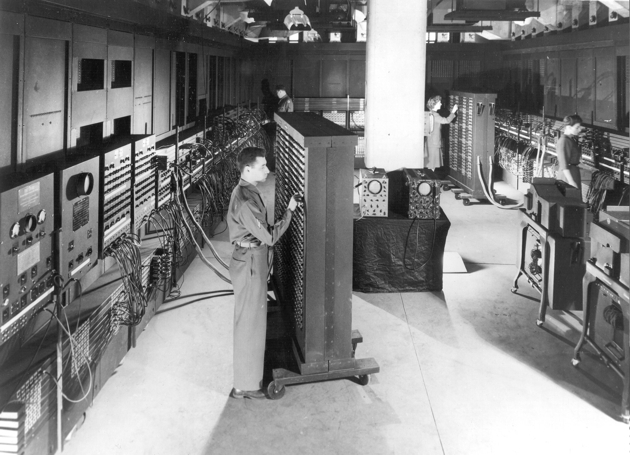
\includegraphics[scale=0.8]{img/eniac.jpg}
  \caption{Cap. Herman Goldstein (în faţă) setează comutatoarele unuia dintre tablourile funcţionale ale ENIAC la Şcoala Moore de Inginerie Electrică. (foto: Armata SUA)}
\end{figure}
\newpage

Transformarea acestuia în mediu a început însă mai târziu. Douglas Engelbart, unul dintre cei care a pus bazele computerelor personale și-a prezentat viziunea de a augmenta inteligența umană cu ajutorul computerelor.

În 1968 Engelbart a prezentat prototipul viziunii sale, numit NLS\footnote{Un sistem complet hardware și software, prescurtare de la "the oN-Line System", }.
Această prezentarea ajuns mai târziu să fie supranumită \textit{Mama tuturor demonstrațiilor}\footnote{În original „Mother of all demos”} deoarece a introdus foarte multe concepte pe care le folosim și astăzi; mouse-ul, ferestrele, interfața grafică, video-conferința, procesarea text, hipertextul, versionarea sau editorul colaborativ în timp real.

Câțiva ani mai târziu Alan Kay a prezentat Dynabook, un prototip al unei platforme colaborative pentru copii.
Un computer portabil cu interfață grafica și touchscreen, capabil de accesare și partajare a informațiilor în rețea. A prezentat o viziune detaliată a tabletelor cu touchscreen decenii înainte să devină practice. Dar mai mult decât o tabletă, el a conceptualizat un mediu dinamic cu care ne putem juca și interacționa.

\begin{figure}[h]
  \centering
  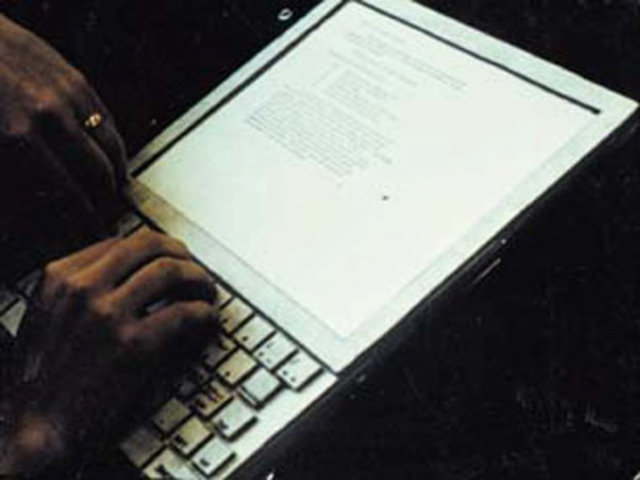
\includegraphics[scale=0.6]{img/dynabook.jpg}
  \caption{Dynabook, dezvoltat și prezentat in 1972}
\end{figure}
\newpage

Aceste concepte perfecționate de-a lungul timpului ne-au adus din ce în ce mai aproape de tehnologie. Dispozitivele electronicele au devenit omniprezente și interconectate. Le purtăm pretutindeni, le putem accesa de la distanță și le putem programa să îndeplinească sarcini în lipsa noastră.

Dar cu toate că am reușit să facem computere mai rapide, mai puternice, mai mici și mai frumoase, modul în care interacționăm cu ele are la bază aceleași concepte introduse acum câteva decenii.

\section{Soluții}

Schimbarea modului în care interacționăm cu tehnologia întâmpină o serie de obstacole de diferite grade de dificultate. Dar pentru a le depăși pe cele mai importante este nevoie de câteva lucruri.

\subsection{Asumarea riscului}

Este cunoscut faptul ca majorității oamenilor le este frica de schimbare. Atâta timp cât confortabila rutină pe care și-au stabilit-o le asigură mijloacele de subzistență, le este frică să se angajeze în ceva ce ar putea eșua, așa că nu încearcă.

Acest lucru este valabil și la nivel de companii, ieșirea din tipar reprezintă un risc prea mare dacă soluția actuală funcționează, fie și la un nivel considerabil sub-optim. Schimbări radicale sau soluții fundamental diferite luându-se în considerare fie în pragul falimentului, fie datorită unei abundențe a resurselor, când costul nu reprezintă o problemă, iar unda șocului eșecului poate fi ușor absorbită.

Asumarea riscurilor este o componentă cheie pentru transformarea în realitate a ideilor revoluționare, pentru inovație.

\subsection{Creativitate}

Procesul de îmbunătățire a tehnologiilor actuale poate fi descris printr-o serie simplă de pași: analizarea dispozitivului în cauză, observarea modului în care este utilizat, găsirea punctelor slabe și concentrarea resurselor asupra găsirii unei soluții, de cele mai multe ori similară, dar mai rapidă și mai eficientă pentru a rezolva aceeași problemă.

Găsirea unor soluții complet noi necesită ieșirea din bula conceptelor deja existente și aplicarea tehnicii de descoperire mai sus menționată.

Un exemplu ce portretizează foarte bine atât creativitatea cât și utilizarea acțiunilor naturale pentru atenuarea curbei de învățare necesar folosirii dispozitivului, este \textit{Robotul telefonic cu biluțe}\footnote{Original \textit{Marble Answering Machine}, "marble" nu are o traducere exactă, sunt biluțe din sticlă, oțel sau agat.}.

\begin{figure}[h]
  \centering
  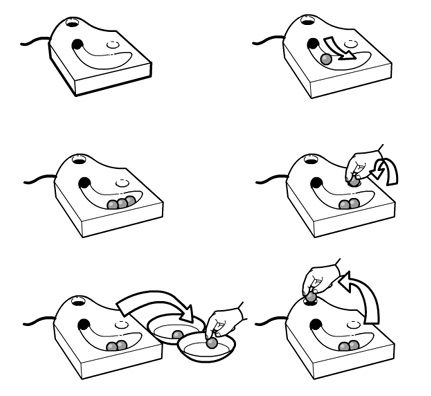
\includegraphics[scale=0.6]{img/marbleAnswMachine.png}
  \caption{Schițe reprezentând modul de utilizare al Robotului telefonic cu biluțe, propus in 1992}
\end{figure}

Robotul telefonic cu biluțe este un prototip proiectat de Durrell Bishop în 1992, și este considerat una dintre primele interfețe cu utilizatorul tangibile sau \textit{TUI}\footnote{TUI, acronim pentru "Tangible user interface"}.
Dispozitivul eliberează o biluță pentru fiecare mesaj vocal primit. Ordinea bilelor indică ordinea în care mesajele au fost recepționate. Mesajele pot fi ascultate plasând biluța corespunzătoare într-un recipient special, salvate prin păstrarea lor fizică, sau șterse prin reintroducerea lor în circuit. Scopul acestui robot telefonic era de a demonstra potențialul de a face informația digitală palpabilă.

\subsection{Uciderea mesagerului}

Comunicarea cea mai eficientă între entități se face atunci când este efectua direct, fără a fi alterată de intermediari.

În cazul interacțiunii omului cu informația digitală acest lucru se poate obține fie prin materializarea acesteia în \textit{metafore palpabile} ca în exemplul biluțelor robotului telefonic, fie prin interacțiune directă cu aceasta în mediul ei natural.
\textit{Realitatea augmentată} ne permite aducerea informației digitale nealterate în lumea reală iar \textit{realitatea virtuală} ne permite să pășim în lumea acesteia.
Dispozitive ca \textit{Leap motion} elimină necesitatea perifericelor ca tastatura, mouse-ul, touchscreen-ul sau joystick-ul, noi înșine devenind „controller-ul”.

\begin{figure}[h]
  \centering
  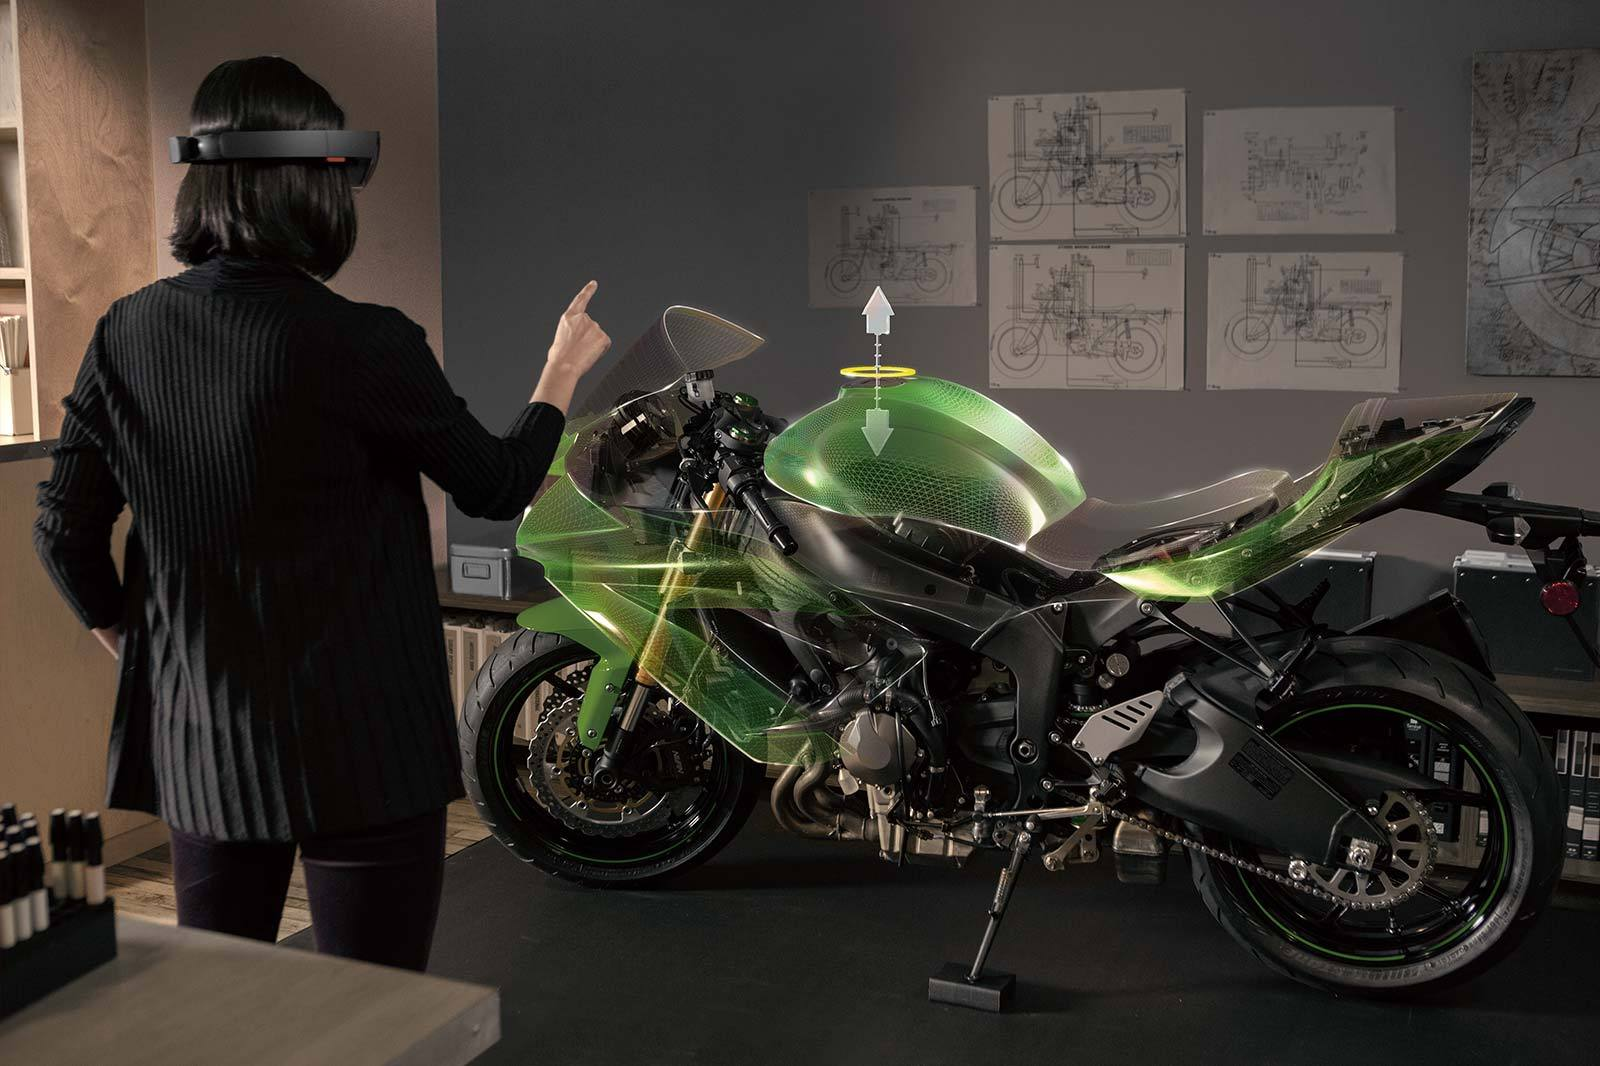
\includegraphics[scale=0.25]{img/microsoft_hololens_demo.jpg}
  \caption{Realitate augmentată, demonstrație a dispozitivului \textit{HoloLens} dezvoltat de Microsoft}
\end{figure}

\cleardoublepage
\chapter {Tehnologii și Spațiu Virtual}

\section{Realitate virtuală}

Transpunerea în pielea diferitor personaje sau în scenarii fictive este ceva ce oamenii fac dintotdeauna. Înainte ca tehnologia să ne permită punerea pe hârtie a gândurilor și fanteziilor, ne adunam și spuneam povești, acest lucru permițându-ne să ne imaginăm pe noi înșine în fiecare din locurile descrise în poveste. Fără ajutorul tehnologiei ne puteam imagina că ne aflăm într-o altă realitate față cea în care ne găseam.

Acest lucru nu poate fi neapărat descris ca realitate virtuală în sensul în care îl folosim astăzi, dar poveștile spuse de mii de ani subliniază faptul că suntem o specie căreia îi place să își folosească mintea pentru a vizita diferite locuri, scenarii și evenimente.
Aceste caracteristici sunt ceea ce n-a împins de-a lungul secolelor să folosim tehnologia pentru a face tranziția în lumi diferite cât mai ușoară, acolo unde doar imaginația nu era de ajuns.

Folosim aceste tehnologii pentru a ne păcăli simțurile în a crede ca suntem altundeva și putem face lucruri incredibile și imposibile de realizat în viața de zi cu zi.

\subsection{Origini}

Tehnologia de \textit{simulare} a unei experiențe datează din 1929 când pionierul în aviație, Edwin Albert Link a inventat un dispozitiv numit \textit{Cutia albastră}\footnote{Original \textit{The blue box}, cunoscut și sub numele de \textit{Link Trainer}}. Era un simulator de zbor  rudimentar, echipat cu motoare pentru a simula rotația avionului pe două axe, utilizat la instruirea piloților în utilizarea comenzilor de bază. Pilotul intra în carlinga închisă izolându-se de exterior. Deși nu avea o reprezentare vizuală a unei lumi virtuale în acest simulator, folosea mișcarea artificială pentru a păcăli simțurile pilotului în a crede că se află într-un avion real.

\newpage

\begin{figure}[h]
  \centering
  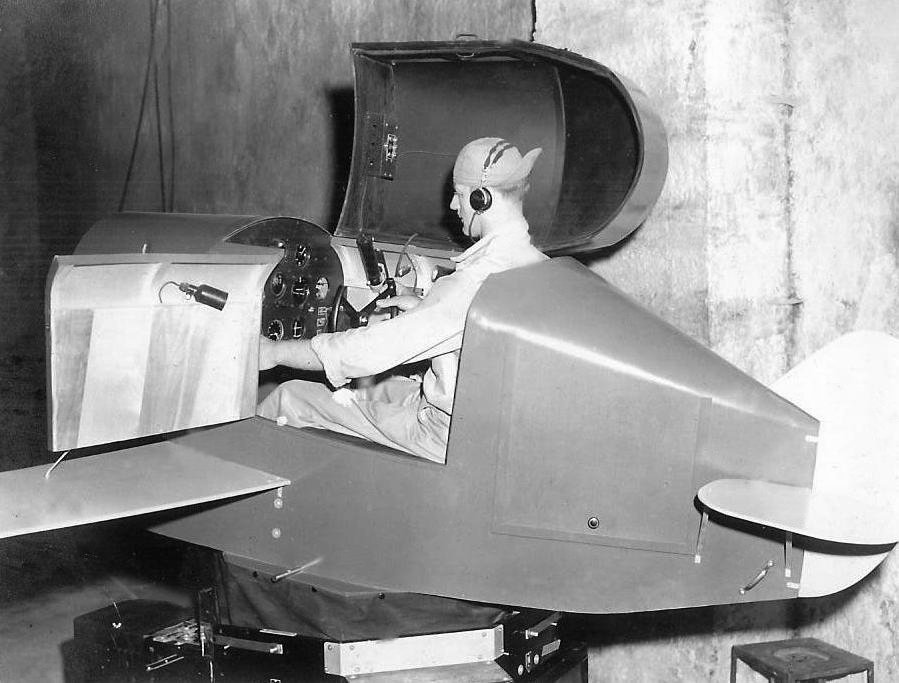
\includegraphics[scale=0.9]{img/link_trainer.jpg}
  \caption{Link Trainer, simulator de zbor inventat în 1929}
\end{figure}


Ceva mai târziu, în 1935 a fost publicată în revista științifico-fantastică \textit{Povestiri fantastice}\footnote{Original \textit{Wonder Stories}}, opera scrisă de Stanley G. Weinbaum intitulată \textit{Ochelarii lui Pygmalion}\footnote{Original \textit{Pygmalion's Spectacles}}.

Aceasta este povestea unui bărbat care primește de la un inventator o pereche de ochelari care îi permiteau purtătorului să ia parte într-o poveste ca și când ar fi cu adevărat prezent în acea lume, putând să vadă, audă, simtă, miroase și să interacționeze cu mediul înconjurător. Nu doar atât, dar purtătorul putea să vorbească personajelor iar acestea răspundeau ca și cum ar fi un alt personaj participând la acțiune.

\textit{Ochelarii lui Pygmalion} este prima mențiune într-o operă literară a ceea ce putem considera ca fiind realitate virtuală și se asemănă izbitor cu dispozitivele VR disponibile astăzi. 
\newpage

Adevăratul pionier al realității virtuale a fost Morton Leonard Heilig, care utilizându-și experiența cinematografică a dezvoltat într-o perioadă de mai mulți ani un aparat numit \textit{Sensorama}, început în 1957 și patentat în 1962.
Sensorama era construit ca jocurile de tip arcade ale anilor '80. Oferea utilizatorului experiența de-a conduce o motocicletă pe străzile din Brooklyn, putea simți vântul pe față, vibrațiile scaunului motocicletei, viziune tridimensională și chiar mirosul orașului.
Heilig a filmat o serie de filme pentru invenția sa, dar din nefericire nu a avut parte de finanțarea necesară pentru Sensorama în producție.

\begin{figure}[h]
  \centering
  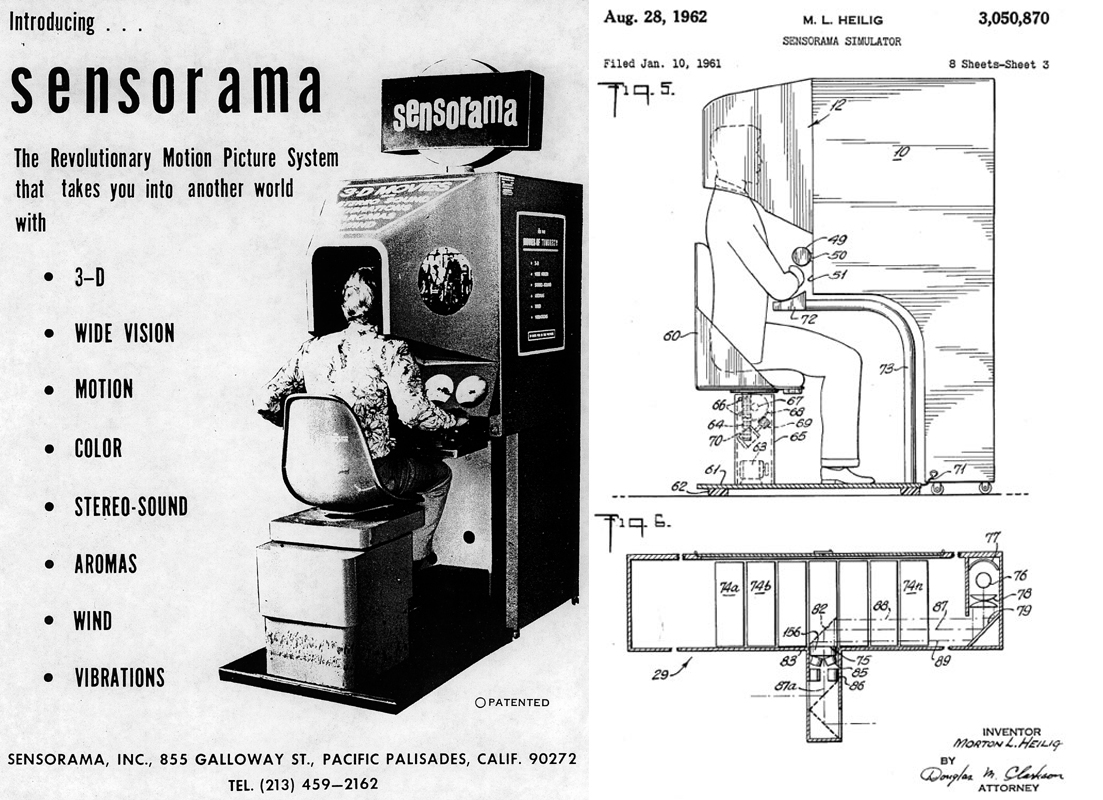
\includegraphics[scale=0.35]{img/sensorama.jpg}
  \caption{Sensorama, dezvoltat între 1957 și 1962}
\end{figure}

\subsection{Realitatea Virtuală în anii '80, '90}

Datorită înaintării progresului tehnologic, realitatea virtuală a făcut salturi uriașe în ani '80 - '90, mulțumită în special interesului dovedit de NASA în acest domeniu.

În 1985 un departament al NASA a dezvoltat \textit{Virtual Environment Display System}, o cască cu ecran stereoscopic și unghi larg de vizibilitate controlat de poziția utilizatorului, vocal și prin gesturi, cu ajutorul unor mănuși speciale.

În 1987 compania \textit{VPL} a creat o serie de tehnologii legate de VR, printre care \textit{Data Glove} și \textit{EyePhone}. VPL a fost prima companie care a comercializat căști de VR și controlere sub formă de mănuși. De asemenea Jaron Lanier fondatorul companiei este cel care a atribuit tehnologiei numele de \textit{realitate virtuală}.

La începutul anilor '90 NASA a transformat \textit{Clădirea 9} din cadrul Centrului Spațial Johnson, într-un spațiu dedicat cercetării și dezvoltării tehnologiei realității virtuale și i-au pus numele de \textit{VR lab}.
Primele căști sau HMD-uri\footnote{\textit{HMD} sau \textit{Head mounted display} este numele atribuit acestor dispozitive, neavând o traducere exactă. Traducerea \textit{ad litteram} ar fi \textit{afișaj montat pe cap} sau, mai intuitiv, \textit{cască}.} folosite de NASA la noul sediu ce cercetare în 1991, foloseau ecrane LCD cu o rezoluție de 320x240 fiind aproape de rezoluția minima a monitoarelor folosite în acea perioadă. Rezoluția acestor ecrane a crescut mult în anii următori, ca în 1994 să ajungă la 1280x1024. 

\begin{figure}[h]
  \centering
  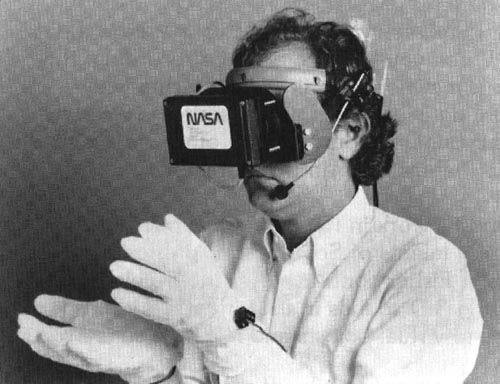
\includegraphics[scale=0.8]{img/nasaVR.jpg}
  \caption{Sistem VR dezvoltat de NASA}
\end{figure}

Una dintre activitățile în care NASA utiliza acest sistem era pentru antrenarea astronauților în folosirea costumelor \textit{EVA}\footnote{\textit{EVA} sau \textit{Extravehicular activity}, tradus ca \textit{activitate extravehiculară}, reprezintă activitățile întreținute de cosmonauți în exteriorul navetelor spațiale, și a atmosferei pământului.} în exteriorul navetelor spațiale.
În aceeași perioadă în care NASA a creat VR lab, o companie debutantă din UK, Virtuality Group a dezvoltat o serie de jocuri arcade. Principalele tipuri de jocuri comercializate erau cele menite să fie jucate din picioare și cele de tip habitaclu. Virtuality a dezvoltat primele versiuni ale elementelor ce se regăsesc în sistemele VR de astăzi, ca senzorii de detectare a mișcării în spațiu, HMD-uri cu timp de răspuns redus și alte inovații software. Căștile aveau două ecrane cu rezoluție de 276x372 și aveau un timp de răspuns de sub 50 de milisecunde.

Aceste jocuri au fost cele care au făcut publicul larg să realizeze potențialul realității virtuale.

\begin{figure}[h]
  \centering
  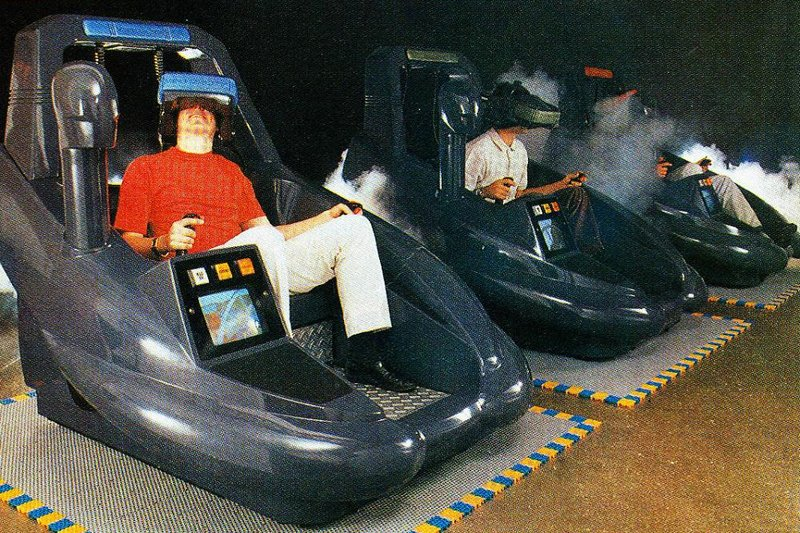
\includegraphics[scale=0.5]{img/virtuality.jpg}
  \caption{Jocuri arcade dezvoltate de Virtuality Group}
\end{figure}

Virtuality nu erau singurii din industria jocurilor interesați de realitata virtuală. SEGA a anunțat SEGA VR în 1991 deși nu a avut un prototip funcțional până în 1993 când a făcut o prezentare la o convenție de electronice. Dar din cauza unor probleme de dezvoltare și a faptului că dispozitivul provoca rău de mișcare și dureri de cap proiectul a fost anulat in 1994.
Nintendo, încercând să profite de interesul publicului pentru aceste tehnologii, a lansat \textit{Virtual boy} în 1995, care deși avea un display stereoscopic nu a fost creat pentru a putea fi purtat pe cap neavând senzori de detectare a mișcării. A fost un eșec comercial abandonat un an mai târziu. 
Un alt proiect abandonat a fost \textit{Jaguar VR,} produs de Atari în colaborare cu Virtuality, colaborare ce nu a fost sustenabilă.

Virtuality Group a continuat să-și dezvolte tehnologia printr-o colaborare cu IBM în 1995, pentru a lucra la așa numitul proiect \textit{Elysium}. Era o stație de lucru pentru PC cu aplicare în arhitectură și construcții.

Alte HMD-uri au mai fost de asemenea lansate în această perioadă, cum ar fi \textit{CyberMaxx} ce avea o serie de jocuri compatibile, ca Doom II și Duke Nukem 3D, dar vânzările au fost extrem de scăzute. \textit{i-glasses!} lansat în 1995, este un alt produs fără succes la vânzări.
\textit{VFX1} era unul dintre cele mai cunoscute astfel de produse ale perioadei, dar din nou, cu succes limitat.

Motivul din spatele eșecului acestor produse se rezumă la puterea de procesare a computerelor și consolelor, ce nu puteau oferi o experiență extraordinară. Din cauza numărului mic de cadre pe secundă combinat cu timpul mare de răspuns, acestea provocau rău de mișcare, dureri de cap și oboseala ochilor. Cu excepția câtorva fani înrăiți, interesul publicului s-a evaporat spre sfârșitul anilor '90.

\subsection{În prezent}

După o perioadă de liniște în lumea realității virtuale, telefoanele mobile au început să încorporeze touchscreen-uri care au ajutat imens la dezvoltarea ecranelor cu rezoluție mare și timp de răspuns tot mai rapid.

Palmer Luckey, antreprenorul care avea să revitalizeze VR-ul, a început ca orice adolescent fascinat de tehnologia realității virtuale colectând și adăugându-și propriile modificări vechilor HMD-uri. Prin intermediul site-ului MTBS3D\footnote{Provine de la \textit{Meant to be seen}, în traducere "trebuie să fie văzut".}, dedicat tehnologiei stereoscopice, a intrat în contact cu John Carmack\footnote{John Carmack este un celebru dezvoltator de jocuri ca, Wolfenstein 3D, Commander Keen, Doom, Quake, Rage.}, care a cerut să-i trimită un prototip.
Carmack și-a adăugat propriile modificări și a prezentat la diverse evenimente unul din primele prototipuri a ce avea sa devină \textit{Oculus Rift}.
În același timp Sony începuse să lucreze la \textit{Project Morpheus} acum cunoscut doar ca Playstation VR. Compania Valve de asemenea a devenit interesată de tehnologie iar printr-un parteneriat cu HTC au dezvoltat HMD-ul cunoscut ca \textit{HTC Vive}.

\begin{figure}[h]
  \centering
  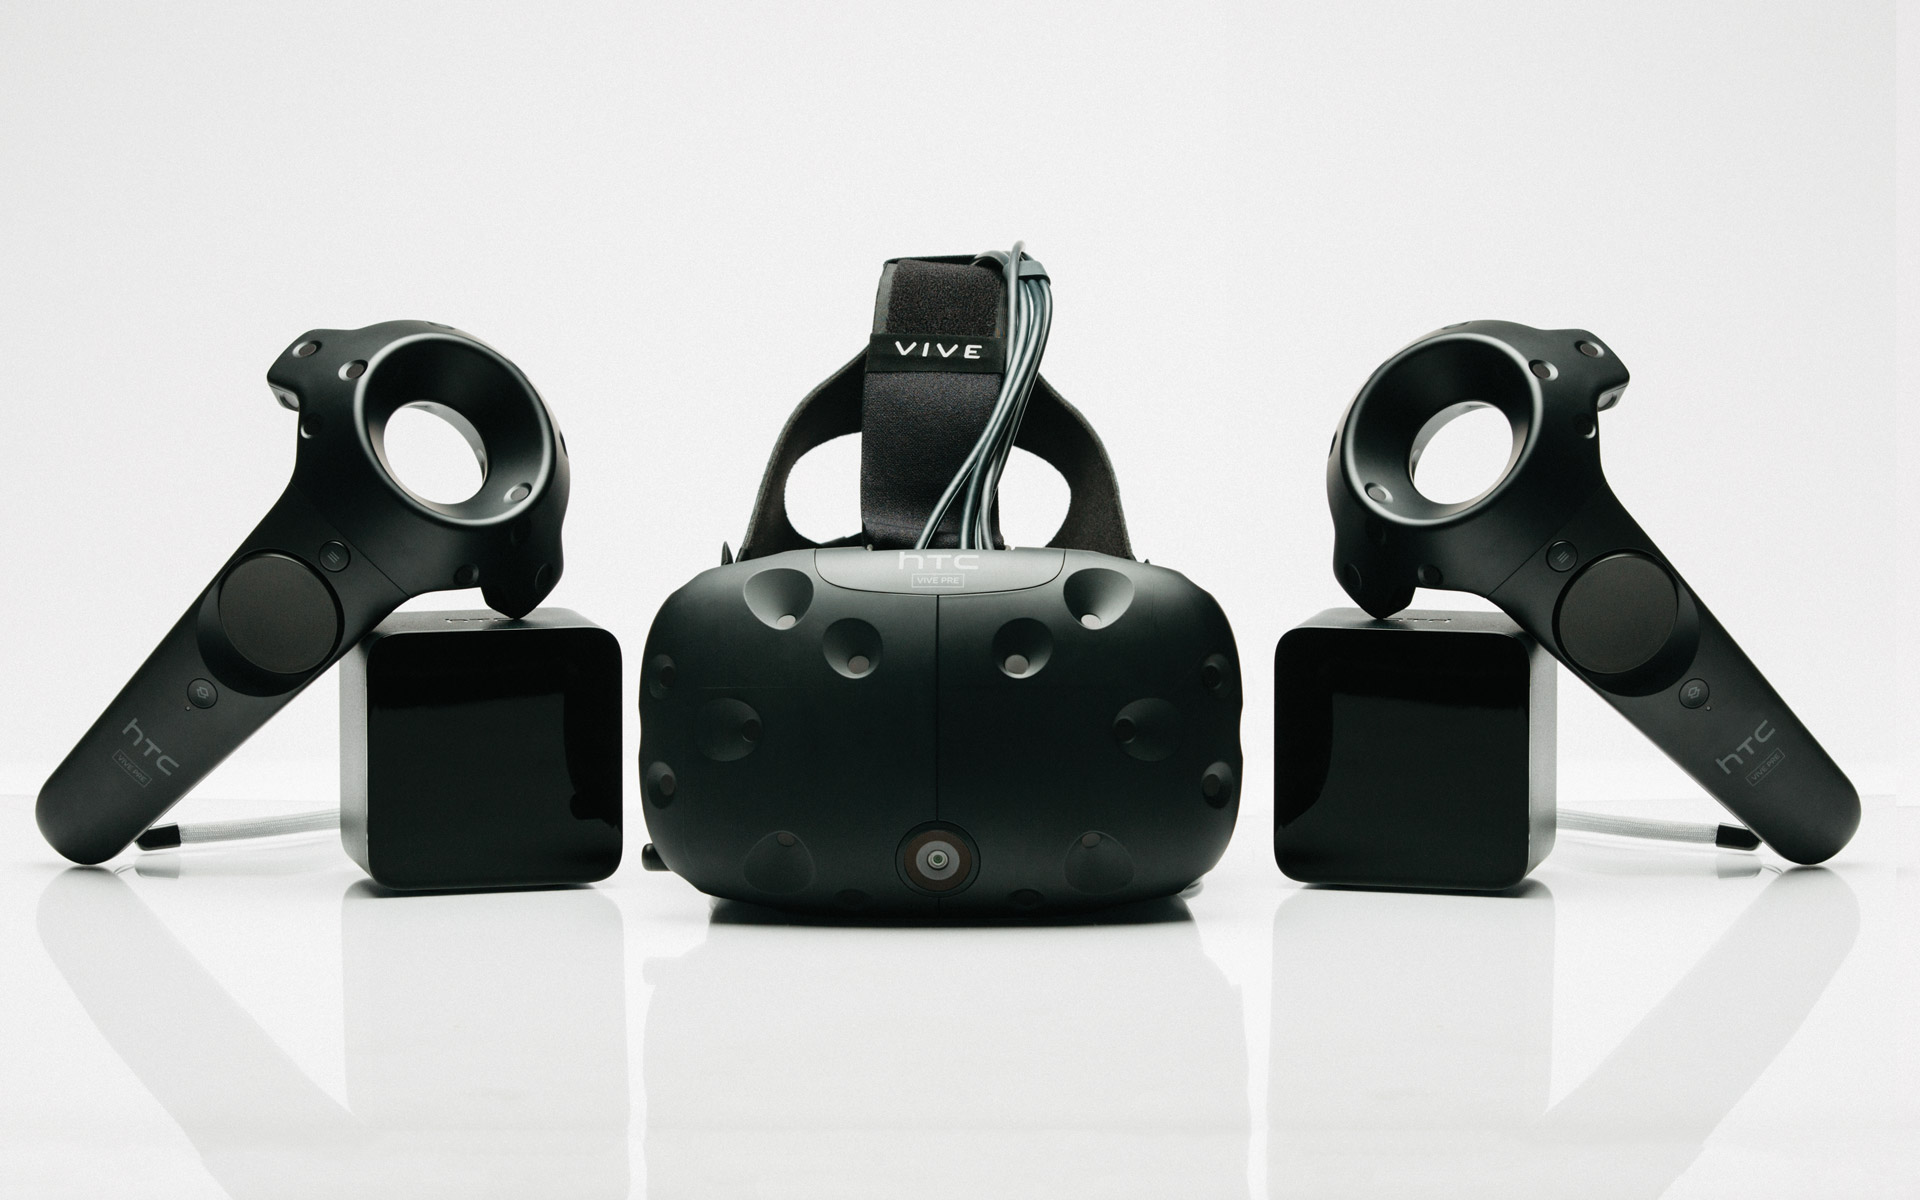
\includegraphics[scale=0.2]{img/htcvive.jpg}
  \caption{Set HTC Vive ce conține cască, controlere și senzori}
\end{figure}

În martie 2014, Facebook a cumpărat Oculus, compania fondată de Palmer Luckey, cu 2 miliarde de dolari și la scurt timp a lansat \textit{Oculus Rif DK2}\footnote{DK2 provine de la \textit{development kit} însemnând kit pentru dezvoltatori.}.

Cele două sisteme pentru PC au fost lansate la o distanță de o săptămână, pe 28 martie 2016 Oculus Rift iar pe 15 aprilie HTC Vive.
\newpage

\subsection{Oculus Rift}

\begin{figure}[h]
  \centering
  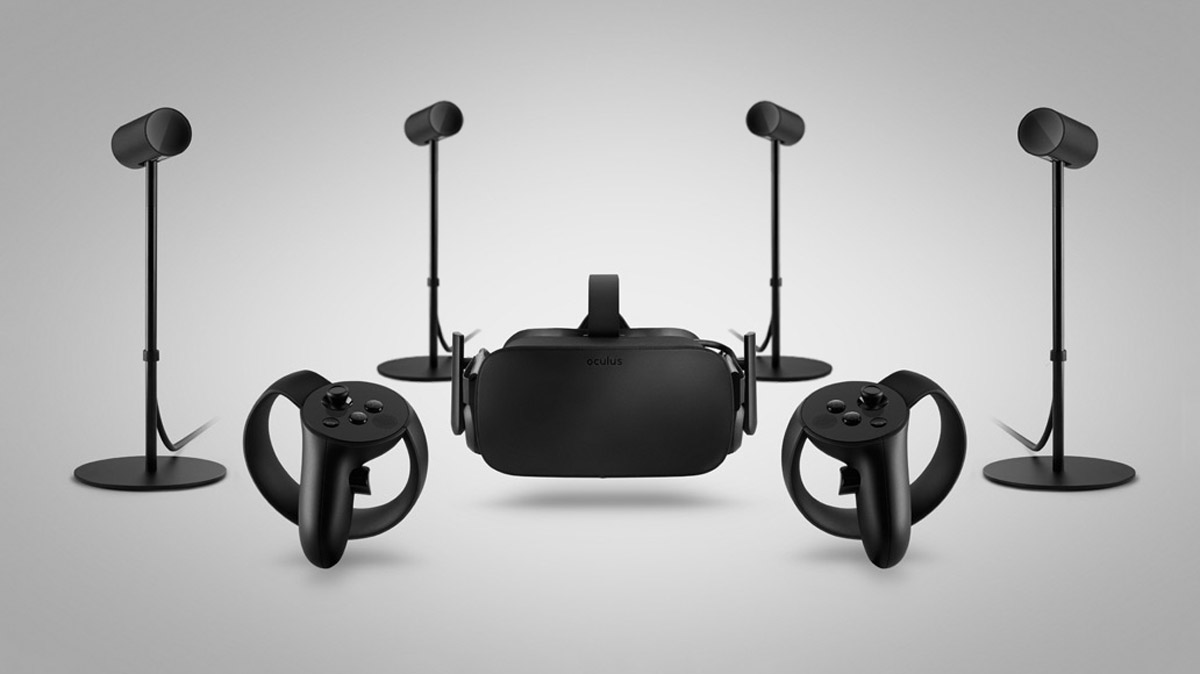
\includegraphics[scale=0.35]{img/oculusRift.jpg}
  \caption{Set Oculus Rift ce conține casca, controlere și senzori}
\end{figure}

De la lansarea campaniei pentru strângere de fonduri pe Kickstarter în 2012 unde a strâns 2,5 milioane de dolari, Oculus a scos două modele de Rift, DK1 și DK2, dedicate programatorilor, ca în martie 2016 să lanseze versiunea pentru publicul larg.
DK1 avea un ecran LCD de 7 inch (18 cm) cu o rezoluție de 1280×800 (format 16:10) ceea ce însemna o rezoluție efectivă de  640×800 pentru fiecare ochi.
DK2 a venit cu o serie de îmbunătățiri, cum ar fi, senzori de detectare a poziției, un ecran OLED cu o rezoluție de 960×1080 pentru fiecare ochi.

Oculus Rift în versiunea sa curentă are câte un ecran OLED pentru fiecare ochi, fiecare cu o rezoluție de 1080×1200, frecvență de 90Hz, și de asemenea persistență redusă, ceea ce înseamnă că afișează o imagine timp de doar 2 milisecunde pentru fiecare cadru.
Folosește lentile care asigură un câmp vizual larg. Lentilele sunt ajustabile pentru a acomoda diferite distanțe interpupilare. Această versiune are încorporată și căști cu efect audio tridimensional.

Sistemul de detectare a poziției, numit \textit{Constellation}, utilizează senzori cu infraroșu ce urmăresc dispozitivele VR. Acestea au LED-uri infraroșu în poziții cheie setate să clipească la o anumită frecvență. Astfel pot determina poziția în spațiu cu o acuratețe sub-milimetrică cu o întârziere ce tinde la zero.

Controlerele de tip \textit{Oculus Touch}, lansate mai târziu, pe 6 decembrie 2016, conțin fiecare câte două butoane trăgaci (eng. \textit{trigger}), două butoane clasice și câte un stick-analog și un sistem de detectare a mișcărilor degetelor.


\section{Prezență virtuală}

Odată intrați în lumea virtuală avem nevoie de o metodă de a putea interacționa cu noul mediu. Desigur, putem continua să folosim tastatura și mouse-ul dar asta nu are prea mult sens în cele mai multe cazuri deoarece ne restricționează libertatea de mișcare, ne afectează imersiunea, iar scopul de a interacționa cât mai natural cu elementele virtuale este complet anihilat.

Din acest motiv dezvoltatorii tehnologiilor VR împerechează HMD-urile cu controlere echipate cu senzori de mișcare, menite să simuleze prezența mâinilor în spațiul virtual, ca \textit{Oculus Touch} menționat anterior, sau \textit{Playstation Move}.
Un alt dispozitiv cu funcția de a transpune mâinile in mediul virtual, dar fără nevoia de a ține un dispozitiv fizic în mână, este \textit{Leap Motion}.

\begin{figure}[h]
  \centering
  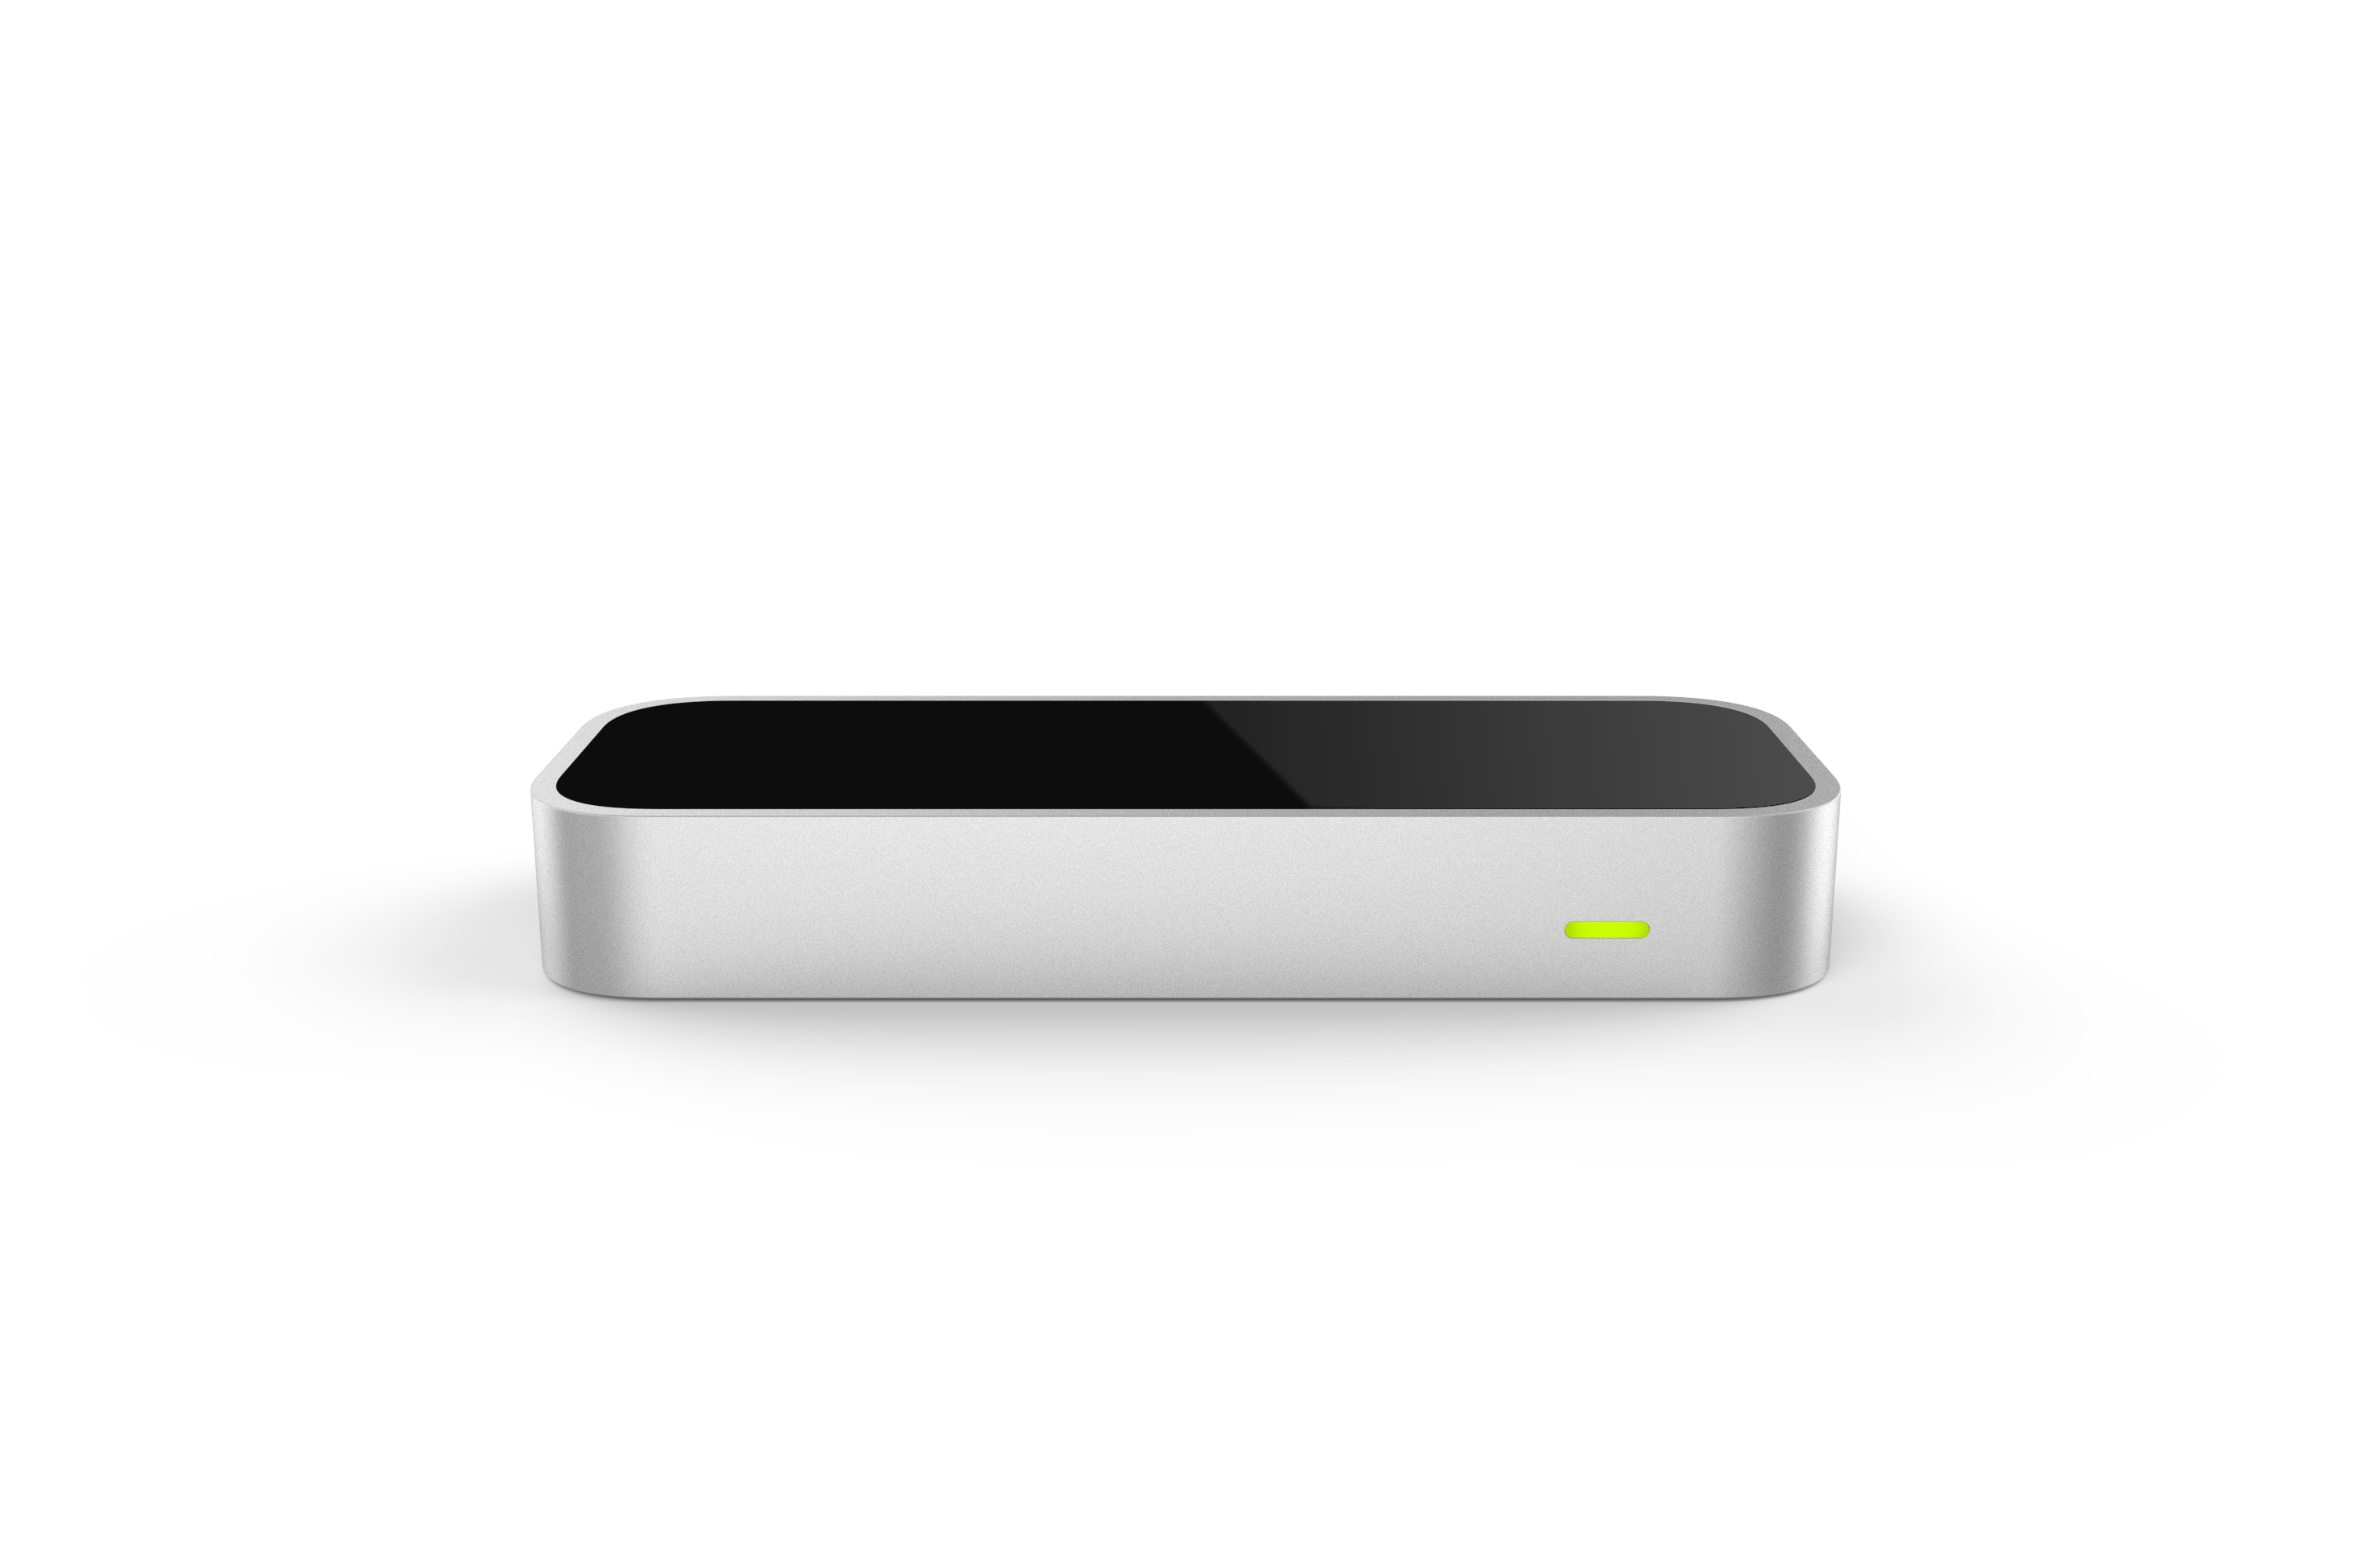
\includegraphics[scale=0.06]{img/LeapMotion.png}
  \caption{dispozitiv Leap Motion}
\end{figure}

Leap Motion este produs de compania americană cu același nume și este un dispozitiv periferic ce poate fi plasat pe o suprafață plată cu fața în sus, sau montat pe parte din față a căștii VR. Folosește două camere cu infraroșu și trei LED-uri infraroșu pentru a observa o zonă aproape semisferică cu raza de aproximativ un metru. LED-urile produc lumină infraroșu continuă, iar camerele generează aproape 200 cadre pe secunda.
Modul exact în care poziția 3D este sintetizată prin compararea celor două imagini 2D generate de camere, nu a fost dezvăluit de companie. Un studiu din 2013 arată că media generală a preciziei cu care controlerul captează și transpune mâinile în obiecte virtuale este de 0,7 milimetri.

\begin{figure}[h]
  \centering
  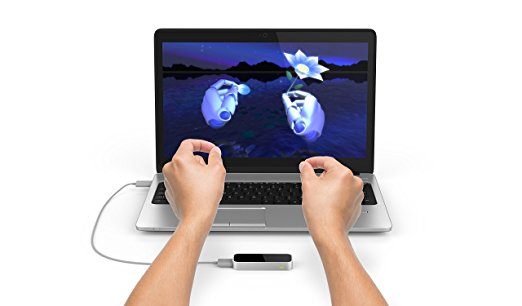
\includegraphics[scale=0.4]{img/leapUse.jpg}
  \caption{dispozitiv Leap Motion în acțiune}
\end{figure}

\section{Unreal Engine}

Un \textit{motor grafic} este un sistem conceput pentru crearea și dezvoltarea de jocuri video. Există mai multe motoare de joc, care sunt proiectate să funcționeze pe console de jocuri video și calculatoare personale. Funcționalitatea de bază oferită de obicei de un motor grafic include un motor de randare\footnote{Din englezescul \textit{renderer}, este rezultatul procesului de preluare și de convertire în imagini a informațiilor digitale introduse într-un mediu programabil de modelare 3D.} pentru grafică 2D sau 3D, un motor de fizică sau de detectare a coliziunilor (și răspunsul la coliziune), sunet, scripting, animație, inteligență artificială, în rețea, streaming, management de memorie, suport de localizare etc. 

\textit{Unreal Engine} este unul din cele mai populare motoare grafice alături de Unity3D, CryEngine, HeroEngine, Rage Engine ș.a.
Dezvoltat de Epic Games, a fost folosit inițial pentru jocul \textit{Unreal} din 1998. Deși conceput pentru jocuri de tip \textit{first-person shooter}\footnote{Tradus \textit{ad litteram} prin \textit{trăgător la prima persoană}, este un gen de joc video în care acțiunea este văzută prin ochii protagonistului.}, este folosit cu succes într-o mare varietate de genuri, printre care \textit{stealth}, \textit{MMORPG-uri}\footnote{\textit{MMORPG}(Massively multiplayer online role-playing game) este o subcategorie a stilului \textit{RPG} (role-playing game) în care jucătorul controlează un personaj inițial slab, dar care pe parcursul poveștii capătă numeroase abilități și în cele mai multe cazuri în funcție de deciziile jucătorului ajunge erou sau antierou, adițional față de RPG, MMORPG-ul este jucat online iar jucătorii pot interacționa atât cu mediul înconjurător cât și între ei.} și alte \textit{RPG-uri}. 

În momentul actual Unreal Engine a ajuns la versiunea 4, care, spre deosebire de versiunile precedente ce rulau cod scris într-un limbaj specific numit \textit{UnrealScript} sau \textit{UScript}, suportă atât programarea în \textit{C++} cât și un sistem de programare vizuală numit \textit{Blueprints Visual Scripting}.

\begin{figure}[h]
  \centering
  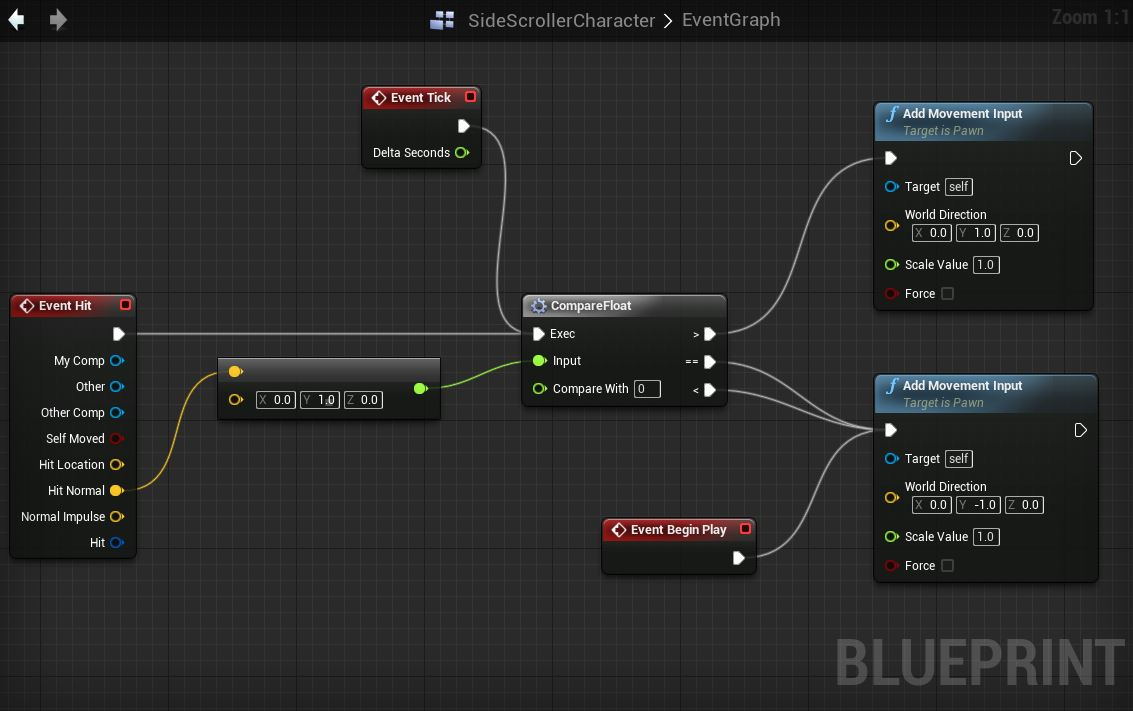
\includegraphics[scale=0.45]{img/simpleBPexample.jpg}
  \caption{Exemplu de script blueprint}
\end{figure}
\newpage
\cleardoublepage
\chapter{Mediu virtual - Particularizare}

Pentru acest proiect am folosit una din versiunile dedicate dezvoltatorilor Oculus Riftu-ului și anume \textit{Developement kit 2}, în combinație cu dispozitivul \textit{Leap Motion} pentru crearea unui mediu virtual în care putem explora o galerie de artă, plasată într-o atmosferă futuristă.

\begin{figure}[h]
  \centering
  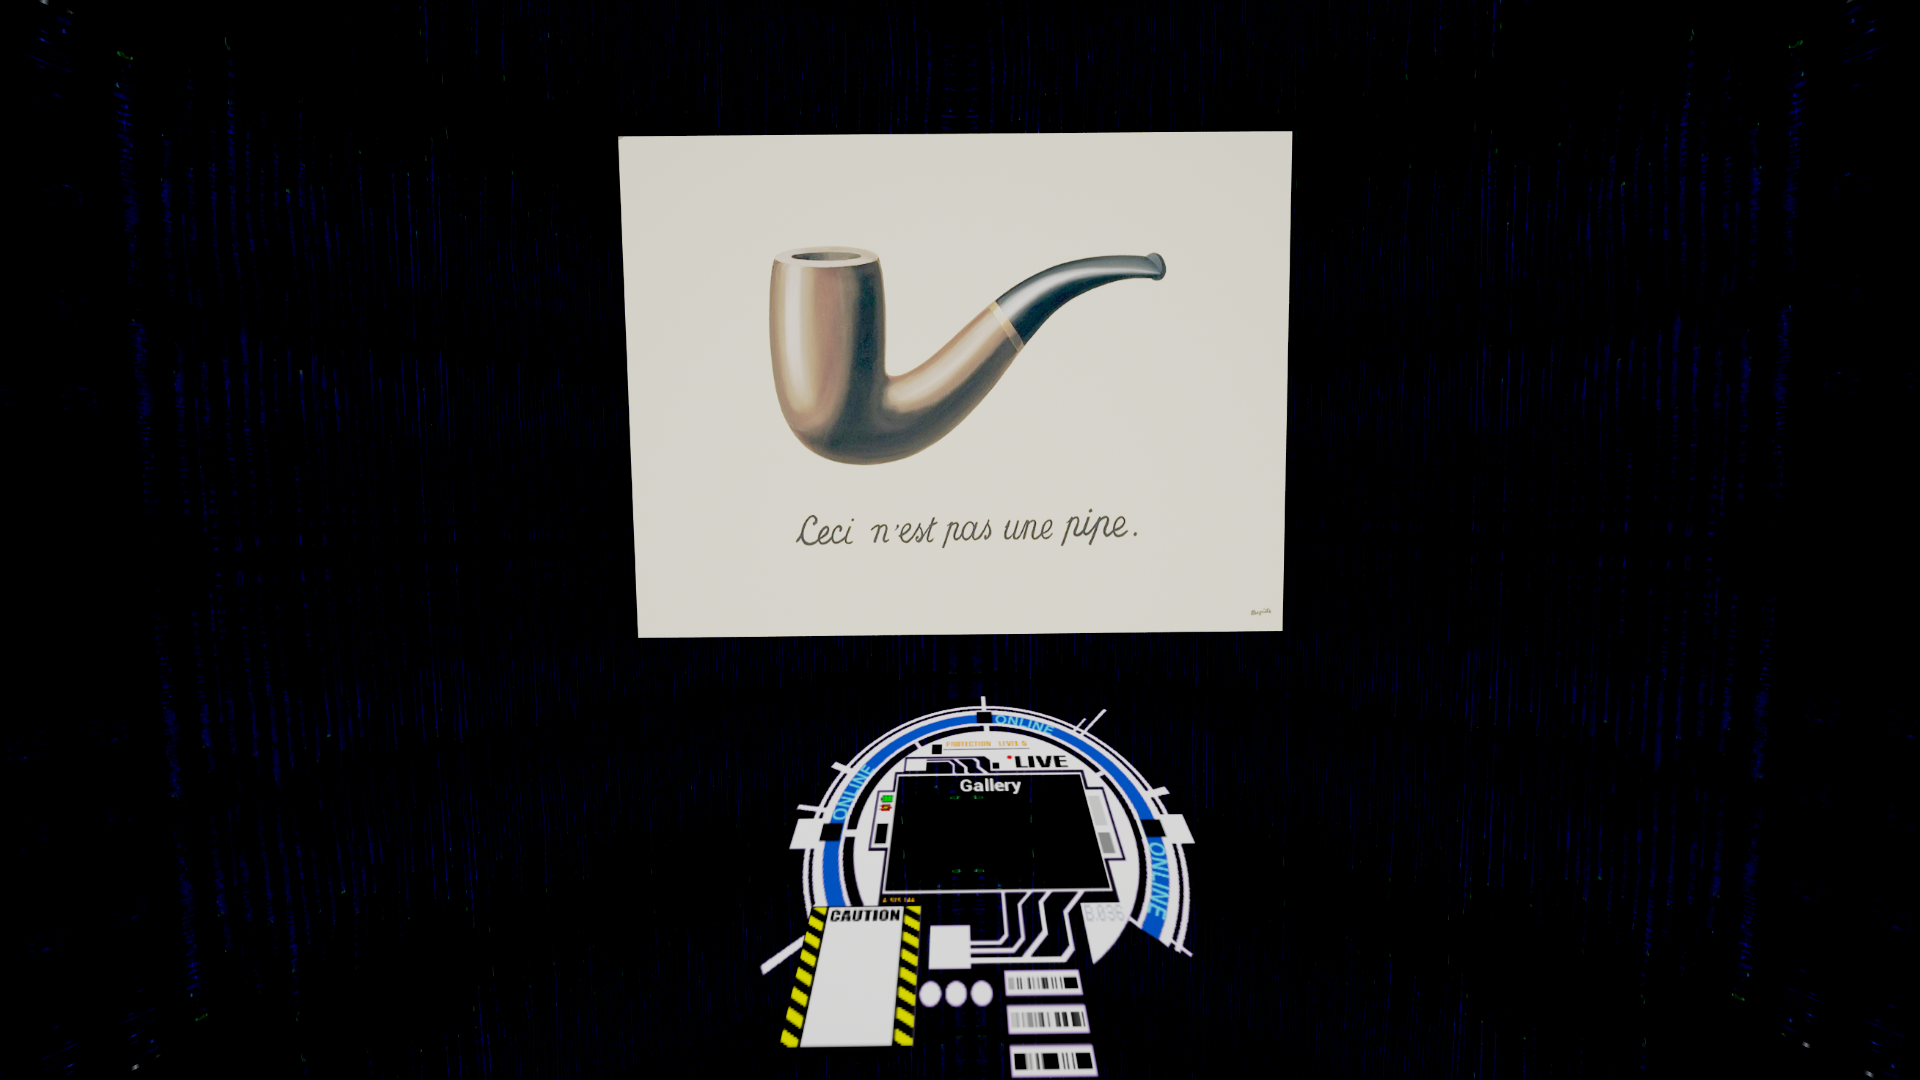
\includegraphics[scale=0.28]{img/screenshot2.png}
  \caption{Captură de ecran al aplicației 3D}
\end{figure}

Ceea ce scoate în evidență prezentarea și explorarea unor elemente într-un spațiu virtual comparativ cu utilizarea browserului într-un plan 2D, este libertatea creatorului de a-și exprima ideile și de a le plasa exact în atmosfera dorită, creând o proiecție a imaginației sale. Imersiunea utilizatorului nu mai este astfel obstrucționată de elemente externe, acesta fiind înconjurat doar de lucruri intenționat plasate.

Există experiențe ce pur și simplu nu pot fi redate prin medii clasice, vizitarea unui muzeu de artă spre exemplu. Deși imaginile picturilor pot fi găsite în cărți sau pe internet, grandoarea operelor este imposibil de capturat prin astfel de medii. Este o experiență complet diferită între a vedea o imagine de câțiva centimetri pe un monitor și de-a o avea în față la dimensiunile unui perete, într-un mediu liniștit fără a fi distras de elemente intruzive.


Un alt caz de utilizare ce poate fi îndeplinit de această aplicație este de a păstra și explora un album foto, acesta putând fi structurat după preferință.
De asemenea în acest mediu pot fi redate și clipuri video,  putând servi ca un cinematograf personal.


Scopul acestei aplicații este de a demonstra un nou mod de interacțiune cu elemente virtuale, prin simpla folosire a mâinilor, un mod de a controla informația digitală folosind cele mai umane și intuitive acțiuni.
De asemenea se exemplifică un mod de explorare a resurselor web în acest mediu, pentru a sublinia potențialul realității virtuale de a deveni un \textit{medium}.

În cazul nostru am folosit platforma XWiki pentru stocarea datelor pe baza cărora se generează principalele elemente grafice din interiorul aplicației.
Din punctul de vedere al utilizatorului aplicația poate fi descompusă în câteva elemente simple: spațiul în care este plasată\footnote{Decorul reprezintă o viziune personală a spațiului cibernetic, cu evidente influențe din \textit{Matrix} și \textit{Ghost in the Shell}.}, niște pseudo-panouri de control cu ajutorul cărora se pot alege și vizualiza operele artistice și proiecția picturii propriu-zise ce poate fi activată sau dezactivată din panoul principal.

Din punct de vedere tehnic, proiecția menționată anterior este un browser web virtual, setat să afișeze imaginile stocate în acest scop pe paginile wiki aferente, panoul principal este o reprezentare a paginii curente, iar cele secundare reprezintă copiii acesteia, afișând doar anumite informații extrase din paginile web.

\begin{figure}[h]
  \centering
  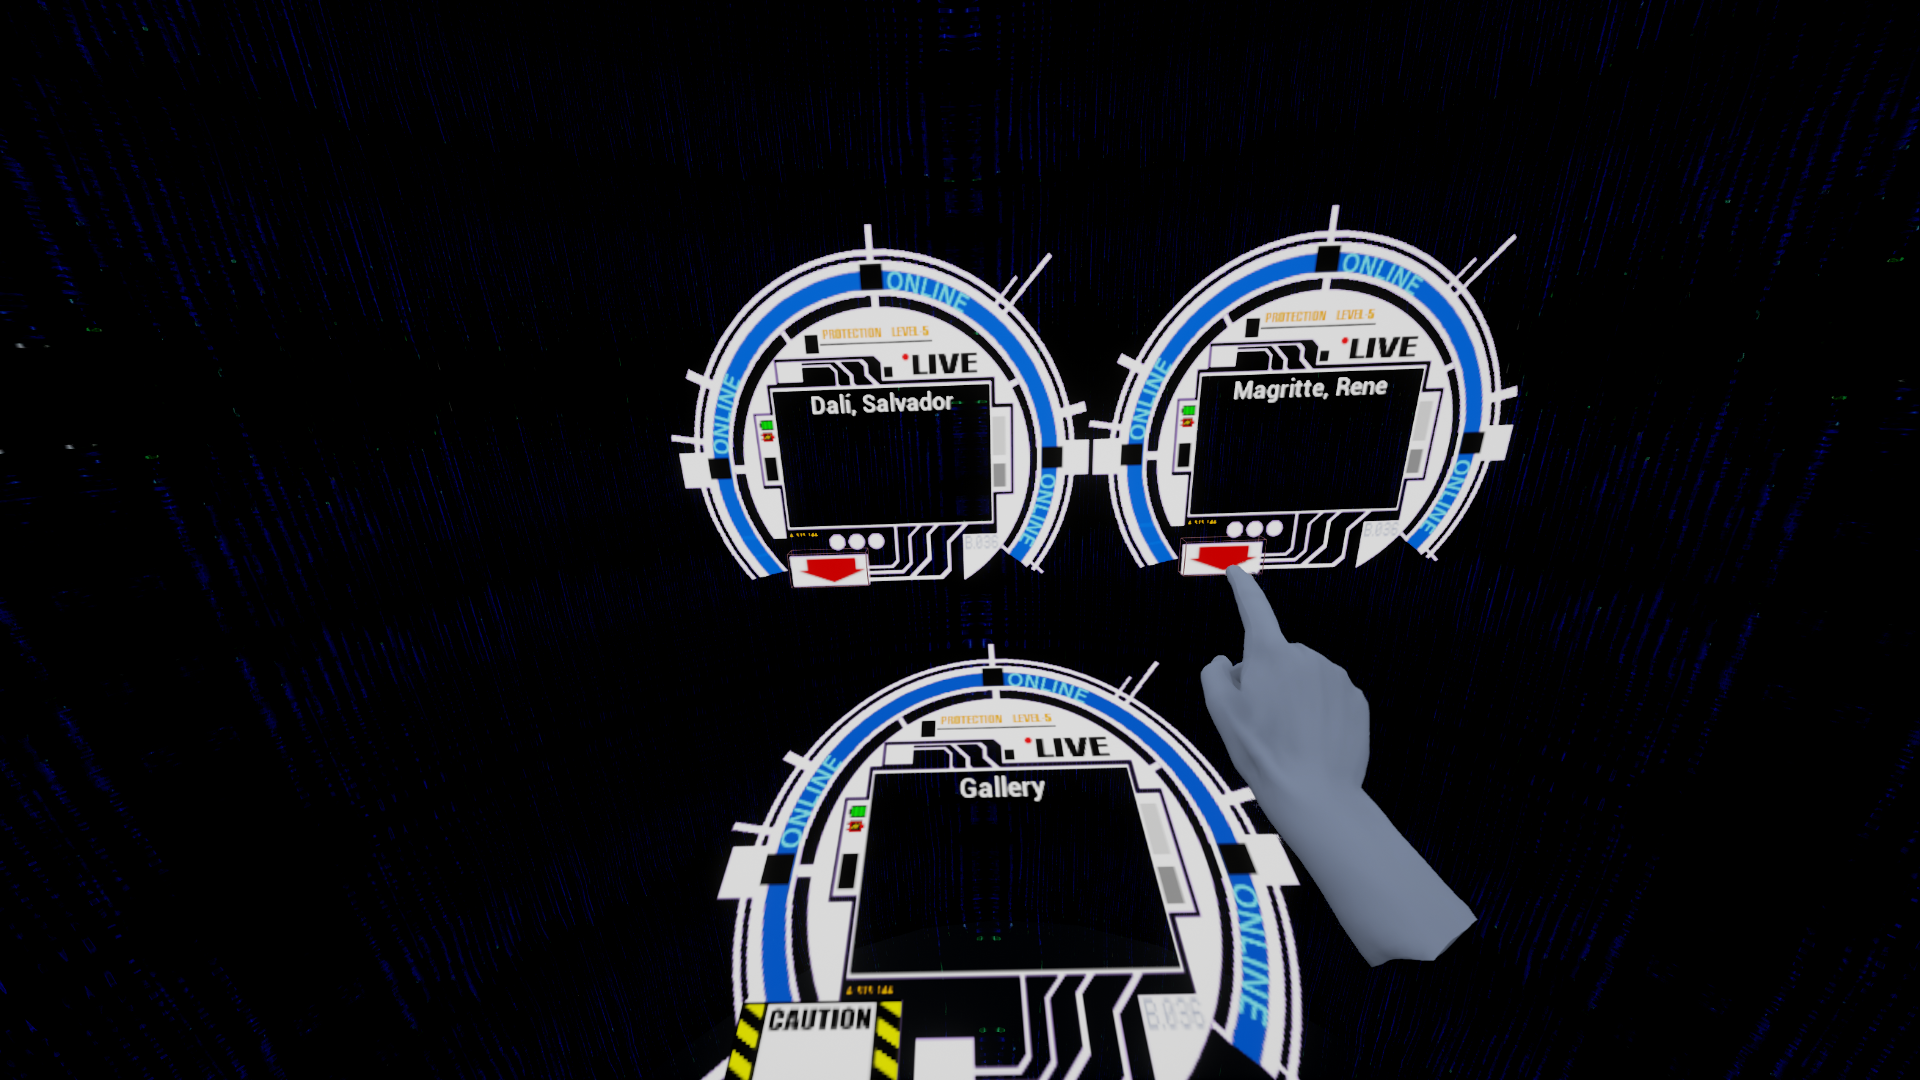
\includegraphics[scale=0.28]{img/screenshot1.png}
  \caption{Captură de ecran a aplicației 3D}
\end{figure}


\section{Implementare}

Pentru implementarea acestei aplicații am ales utilizarea motorului grafic \textit{Unreal Engine}, versiunea 4.12, datorită suportului pentru dispozitivele Oculus Rift și Leap Motion, și a comunității mari și active de utilizatori.

Pentru afișarea tridimensională pe ecranul căștii de realitate virtuală, și utilizarea senzorilor de mișcare ale acesteia am folosit plugin-urile \textit{Oculus Rift} și \textit{biblioteca Oculus}, oferite de Unreal Engine.

Realitatea virtuală păcălește creierul în a crede ca te afli într-o lume tridimensională, efect creat de un afișaj stereoscopic. Acest lucru funcționează afișând câte o imagine, pentru fiecare ochi, a aceleiași scene din două unghiuri ușor diferite, simulând distanța.

\begin{figure}[h]
  \centering
  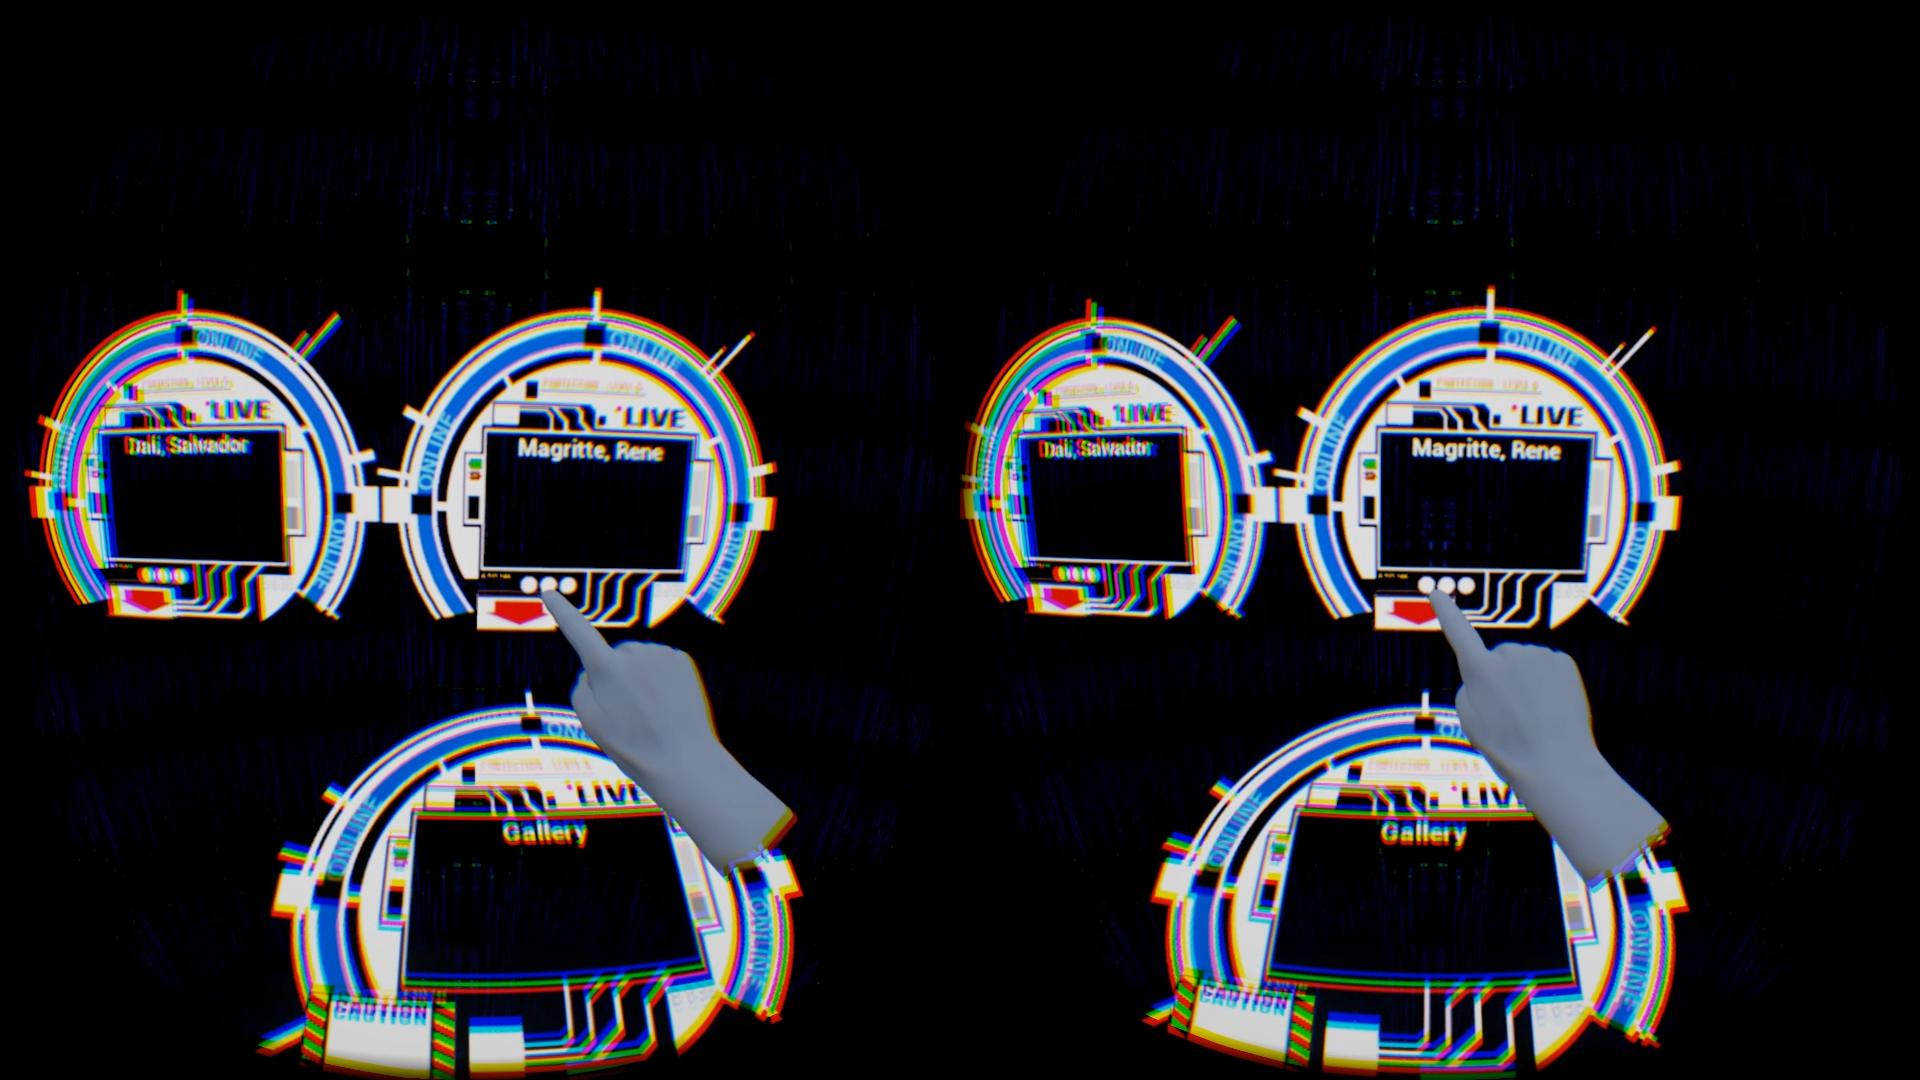
\includegraphics[scale=0.28]{img/stereoscopic.png}
  \caption{Afișaj stereoscopic ce crează efetul de distanță}
\end{figure}

Pentru captura și transpunerea mâinilor în spațiul virtual cum este observabil și în imaginea de mai sus, am utilizat plug-inul \textit{Leap Motion}, ce vine cu o varietate de opțiuni în ceea ce privește caracterul principal, ce funcționează împreună cu Oculus Rift, cum ar fi simularea unui corp a cărui mâini pot fi controlate cu Leap Motion, iar camera (punctul de vedere al jucătorului) va fi la nivelul ochilor acestui caracter, sau un caracter ce are doar mâinile prezente, în stilul jocurilor \textit{First-person shooter}. 
În cazul nostru am ales \textit{LeapFloatingHandsCharacter}, un caracter imaterial în care mâinile vor fi prezente doar în cazul detecției de către dispozitivul Leap Motion. Acest Plug-in ne oferă și posibilitatea de a face diferite acțiuni folosind gesturi ale mâinii ca metodă de input, spre exemplu pentru a putea vedea mai bine picturile, putem strânge pumnul stâng iar panourile vor dispărea. Repetarea mișcării le va aduce înapoi.


În ceea ce privește implementarea propriu-zisă, după cum am menționat anterior, Unreal Engine oferă atât posibilitatea utilizării unui limbaj vizual de scripting cât și programarea în limbajul C++.
Aici am folosit o combinație intre aceste moduri, sistemul de blueprint-uri pentru implementarea elementelor grafice și stabilirea interacțiunilor dintre ele, iar C++ pentru accesarea documentelor XWiki, parsarea XML-urilor returnate în urma apelurilor REST, și modificarea URL-urilor după caz.

\subsection{Blueprint-uri}

Am început prin a crea într-un spațiu gol, mediul ambiant ce este constituit dintr-o sferă goală, translucidă în centru căreia se află o platformă de sticla pe care stă personajul.
Sfera este la bază ceea ce în limbajul motoarelor grafice se numește un \textit{actor}\footnote{Un obiect ce poate fi plasat spațiul tridimensional, ce suportă transformări cum ar fi \textit{translație, scalare} sau \textit{rotație}} de tip \textit{static mesh}\footnote{Formă geometrică construită dintr-un set de poligoane ce este stocată în memoria video și randată de placa video}, asupra căreia am aplicat o serie de personificări pentru a crea efectul că informația digitală ne înconjoară fizic.

Acest efect a fost obținut prin crearea unui \textit{material}\footnote{Element ce poate fi aplicat unui \textit{mesh} pentru a-i schimba aspectul vizual} special format dintr-o imagine clasică, un negativ al imaginii (utilizat pentru obținerea transparenței) și un set de reguli pentru a dinamiza materialul.

\begin{figure}[h]
  \centering
  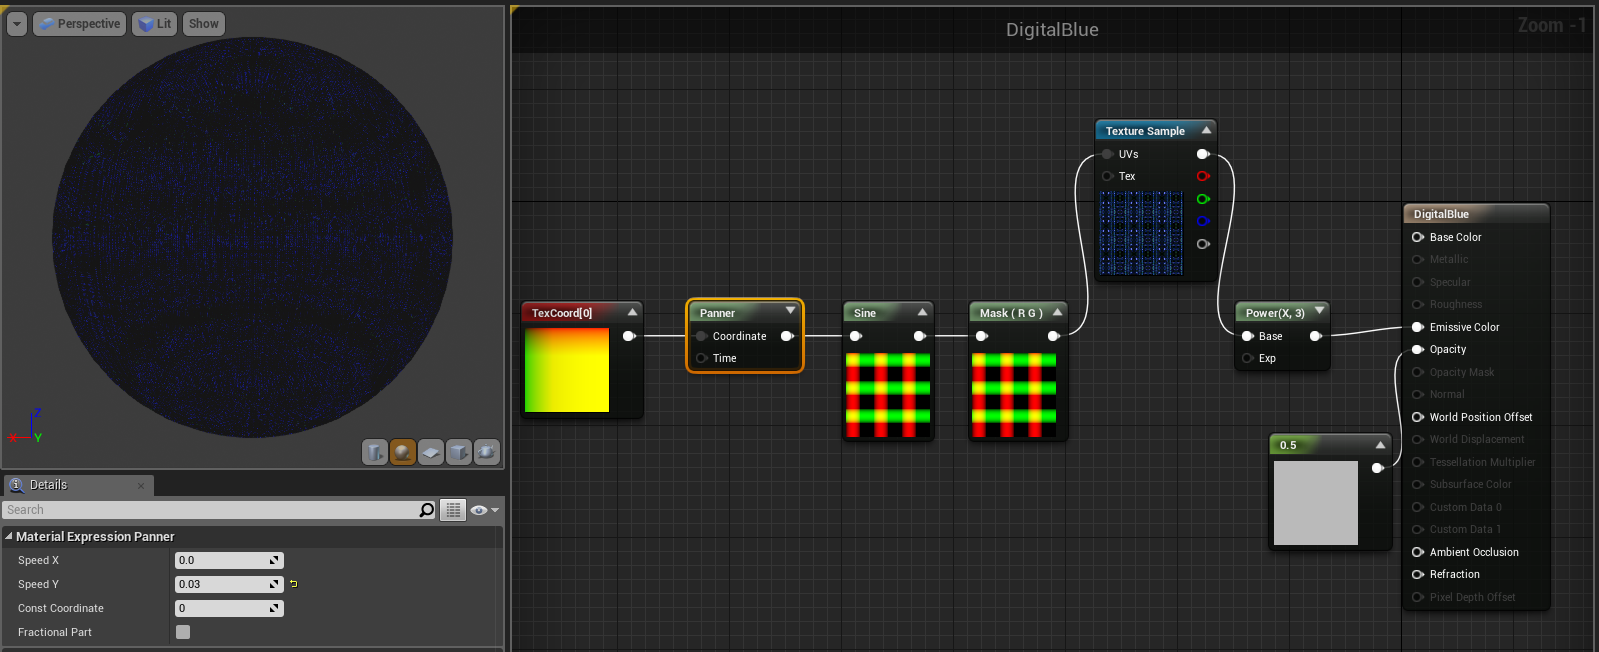
\includegraphics[scale=0.33]{img/digitalBlue.png}
  \caption{Blueprint ce conține regulile materialului dinamic aplicat sferei ambientale}
\end{figure}

Elementele interactive au fiecare asociate câte un \textit{actor} și un \textit{widget blueprint}.
Ecranul digital pe care afișăm imaginile este constituit dintr-un widget blueprint ce are la bază un \textit{canvas} în care este încărcat un browser web, și actorul ce are drept \textit{componentă}\footnote{Un tip special de obiect menit să fie utilizat ca sub-obiect în interiorul unui \textit{actor}. Sunt în general utilizate acolo unde este nevoie de părți modificabile.} widget-ul, căruia i se stabilesc niște setări de afișaj. Actorul primește ca parametru URL-ul imaginii pe care o va afișa browserul și implementează o funcție de schimbare a stării de vizibilitate a acestuia.
\newpage

\begin{figure}[h]
  \centering
  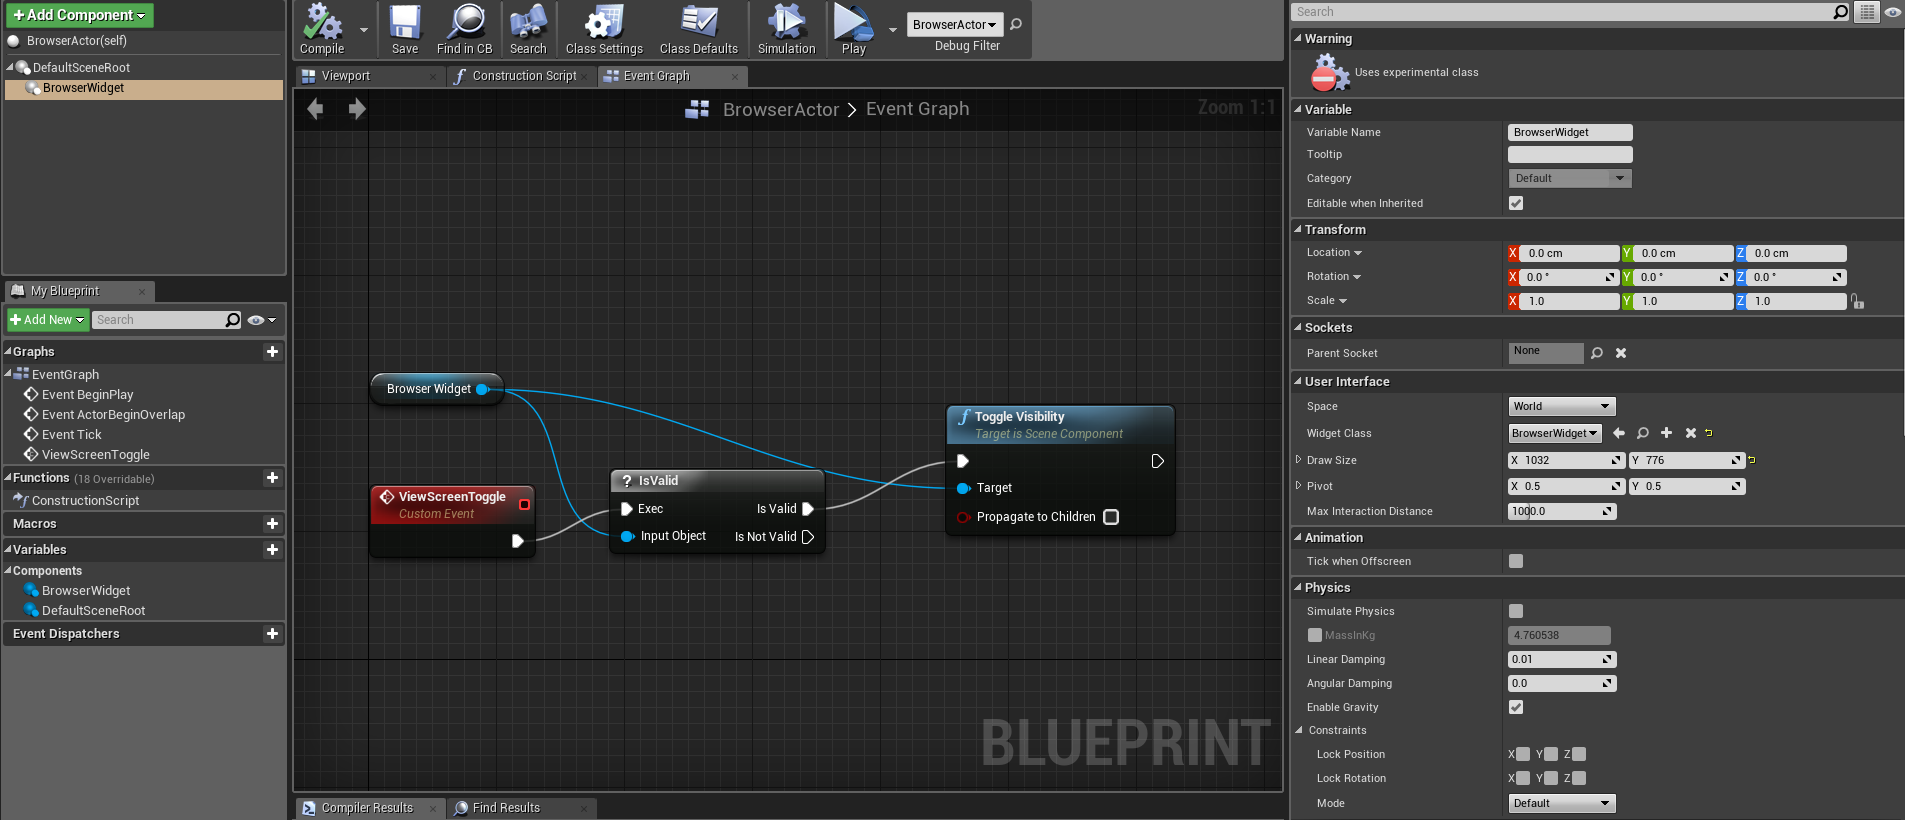
\includegraphics[scale=0.28]{img/toggleVisBrowserActor.png}
  \caption{Funcția de schimbare a stării de vizibilitate implementată de \textit{browser actor}}
\end{figure}
 
Panoul principal din fața utilizatorului este o instanță a unui actor ce conține mai multe componente: un \textit{widget} în care se găsesc o imagine și un bloc text, conținute de un canvas; \textit{LeaptController} componentă de care avem nevoie pentru a putea face referință la \textit{LeapRiggedEchoHeandsActor}, actorul ce reprezinta mâinile virtuale implementat de plug-in-ul \textit{Leap Motion}; și \textit{treeNodeComponent} ce este o clasă C++ în care procesăm paginile web și la care vom reveni ceva mai târziu.

Acest panel are două roluri importante, afișează informații despre pagina curentă și transmite către \textit{BrowserActor} (ecranul în care afișăm imaginile), URL-ul primei imagini din pagina curentă marcate ca fiind \textit{pictură} sau \textit{fotografie}.
Pentru a vedea cum sunt afișate și actualizate informațiile în blocul text al panelului trebuie șă analizăm următoarele scripturi implementate de actorul panelului.

\begin{figure}[h]
  \centering
  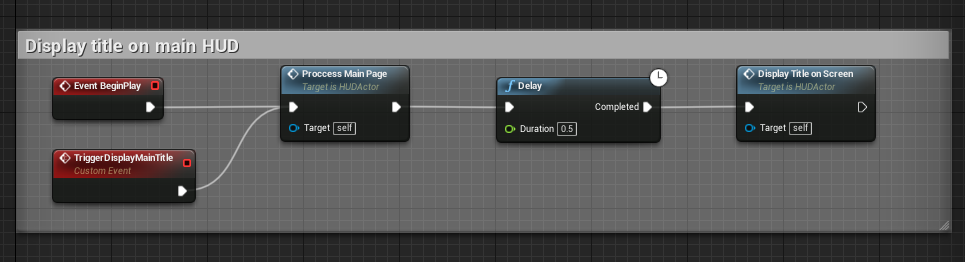
\includegraphics[scale=0.55]{img/DisplayTitleScript1.png}
  \caption{Scriptul principal de afișare a titlului în ecranul panelului}
\end{figure}

\textit{Event BeginPlay} este o funcție standard ce marchează începutul rulării programului, iar \textit{TriggerDisplayMainTitle} este un eveniment personalizat ce este apelat de utilizator când accesează o pagină copil. Ambele evenimente declanșează funcția \textit{ProccessMainPage}, ce apelează componenta C++ responsabilă cu procesarea paginii web și va actualiza lista cu informații selectate din aceasta, dupa care funcția \textit{DisplayTitleOnScreen} va seta valoarea textului afișat, în funcție de informația primită.
\newpage

\begin{figure}[h]
  \centering
  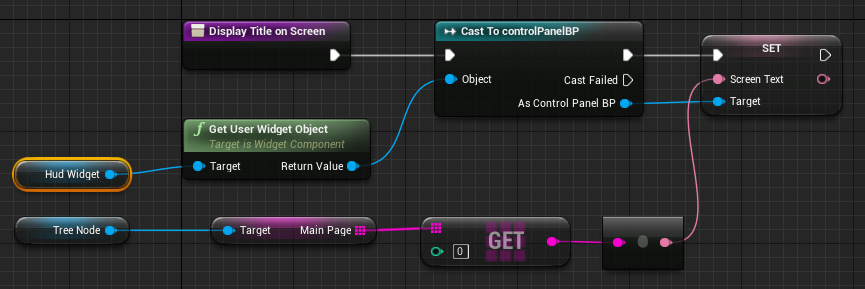
\includegraphics[scale=0.6]{img/DisplayTitleScript2.png}
  \caption{Conținutul funcției \textit{DisplayTitleOnScreen}}
\end{figure}

În figura 3.7 observăm conținutul funcției de afișare/actualizare a titlului paginii principale. Ramura de jos reprezintă lista cu informații despre pagina curentă returnată de componenta \textit{TreeNode} din care se selectează doar elementul cu indexul 0 ce întotdeauna va reprezenta titlul paginii. Acest element va deveni valoarea variabilei \textit{ScreenText} afișate de widget (\textit{controlPanelBP}).

Panourile secundare cu care utilizatorul poate interacționa pentru a selecta printre copii paginii curente au o construcție similară cu panoul principal cu excepția faptului că nu au un loc fix în spațiu. Ele sunt generate în fața utilizatorului pe baza informație primite în urma procesării paginii principale. Fiecare panou are asociate informații referitoare la pagina copil pe care o reprezintă, obținute prin folosirea API-ului REST oferit de platforma XWiki.

Actorul acestor panouri conține în principiu aceleași componente ca cel al panoului principal, \textit{TreeNode} pentru a avea acces la lista cu date despre pagina pe care o reprezintă, \textit{LeapController} pentru ca utilizatorul să le poată muta sau apăsa butoanele acestora, dar o diferență importantă este că acesta conține un container în care widget-urile vor fi generate ca sub-componente a acestuia în funcție de numărul copiilor paginii curente.
În urma selectării unuia dintre copii, URL-ul asociat acestuia va fi încărcat și procesat acesta devenind pagină principală iar lista componentelor va fi actualizată.


\begin{figure}[h]
  \centering
  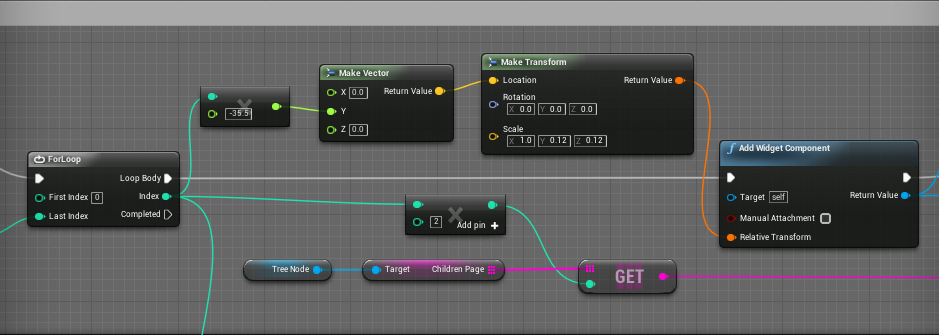
\includegraphics[scale=0.55]{img/SnipetTransform.png}
  \caption{Snippet din scriptul actorului \textit{ChildActor} responsabil cu calcularea pozițiilor în spațiu a panourilor generate}
\end{figure}

\subsection{C++}

În ceea ce privește programarea C++, se poate face din IDE-ul preferat, iar în acest caz am ales Visual Studios 2015 datorită suportului nativ și a funcției de \textit{hot reload}.
API-ul de gameplay și clasele framework-ului Unreal sunt accesibile atât sistemului vizual de scripting cât și din C++.

Aici am utilizat C++ pentru crearea componentei \textit{TreeNodeComponent} de care am vorbit în secțiunea anterioară ce are rolul de a accesa, selecta și aduce informații relevante din documentele XWiki.
Această componentă face disponibile câteva lucruri pe care le accesăm din blueprint-urile discutate mai sus.

\begin{lstlisting}[breaklines=true, postbreak=\mbox{\textcolor{red}{$\hookrightarrow$}\space}, caption=Snippet din fișierul header al componentei \textit{TreeNode} în care sunt declarate componentele esențiale utilizate în blueprint-uri]
public:	
	FHttpModule* Http;

	/* The actual HTTP call */
	UFUNCTION()
		void accessWebsite(FString urltoaccess);
	UFUNCTION(BlueprintCallable, category="WebAccess")
		void proccessURL(FString crtUrl);

	//Create children url from main url
	FString ConstructChildrenUrl(FString crtUrl);

	/*Assign this function to call when the GET request processes sucessfully*/
	void OnResponseReceived(FHttpRequestPtr Request, FHttpResponsePtr Response, bool bWasSuccessful);

	// Sets default values for this component's properties
	UTreeNodeComponent();

	// Called when the game starts
	virtual void BeginPlay() override;
	
	// Called every frame
	virtual void TickComponent( float DeltaTime, ELevelTick TickType, FActorComponentTickFunction* ThisTickFunction ) override;

	UPROPERTY(Category = CustomElements, EditAnywhere, BlueprintReadWrite)
		FString crtChildrenUrl;

	UPROPERTY(Category = CustomElements, EditAnywhere, BlueprintReadWrite)
		TArray<FString> mainPage;

	UPROPERTY(Category = CustomElements, EditAnywhere, BlueprintReadWrite)
		TArray<FString> childrenPage;
\end{lstlisting}

\textit{crtChildrenUrl} este adresa la care găsim informații referitoare la copii paginii curente, iar \textit{mainPage} și \textit{childrenPage} sunt liste ce conțin informații precise ca titlul, conținutul, adresa pentru pagina principala respectiv copii acesteia.

Pentru accesarea paginilor web am folosit biblioteca \textit{Http.h} iar pentru procesarea xml-urilor returnate am folosit bibliotecile \textit{XmlParser} și \textit{FastXml}, toate oferite de framework-ul Unreal.

Funcția \textit{accessWebsite} efectuează apelul http efectiv al cărei răspuns este procesat ulterior iar informațiile relevante sunt extrase și adăugate în listele corespunzătoare.

\begin{lstlisting}[breaklines=true, postbreak=\mbox{\textcolor{red}{$\hookrightarrow$}\space}, caption=Funcția ce efectuează apelul http]
/*Http call*/
void UTreeNodeComponent::accessWebsite(FString urltoaccess)
{
	TSharedRef<IHttpRequest> Request = Http->CreateRequest();
	Request->OnProcessRequestComplete().BindUObject(this, &UTreeNodeComponent::OnResponseReceived);
	//This is the url on which to process the request
	Request->SetURL(urltoaccess);
	Request->SetVerb("GET");
	Request->SetHeader(TEXT("User-Agent"), "X-UnrealEngine-Agent");
	Request->SetHeader("Content-Type", TEXT("application/xml"));
	Request->ProcessRequest();
}
\end{lstlisting}

\begin{lstlisting}[breaklines=true, postbreak=\mbox{\textcolor{red}{$\hookrightarrow$}\space}, caption=Codul funcție principale ce este apelabilă din scripturile blueprint]
void UTreeNodeComponent::proccessURL(FString crtUrl) {
	mainPage.Empty();
	childrenPage.Empty();
	crtUrl = crtUrl + "?xpage=xml";
	crtChildrenUrl = ConstructChildrenUrl(crtUrl);
	accessWebsite(crtUrl);
	accessWebsite(ConstructChildrenUrl(crtUrl));
}
\end{lstlisting}

\begin{lstlisting}[breaklines=true, postbreak=\mbox{\textcolor{red}{$\hookrightarrow$}\space},caption={Funcția ce parsează xml-ul returnat de \textit{http request}, și adaugă informații în listele menționate anterior}]
/*Assigned function on successfull http call*/
void UTreeNodeComponent::OnResponseReceived(FHttpRequestPtr Request, FHttpResponsePtr Response, bool bWasSuccessful)
{
	if (bWasSuccessful) {
		if (Request->GetURL().EndsWith("xpage=xml"))
		{
			//Load xml for main pages
			const FString XWNodeString = Response->GetContentAsString();
			FXmlFile * File = new FXmlFile(XWNodeString, EConstructMethod::ConstructFromBuffer);
			FXmlNode* pRoot = File->GetRootNode();

			FXmlNode* titleNode = const_cast<FXmlNode*>(pRoot->FindChildNode("title"));
			FString pageTitle = titleNode->GetContent();
			FXmlNode* contentNode = const_cast<FXmlNode*>(pRoot->FindChildNode("content"));
			FString pageContent = contentNode->GetContent();
			mainPage.Add(pageTitle);
			mainPage.Add(pageContent);

			File->Clear();
		}
		else if (Request->GetURL().EndsWith("pages/WebHome/children")) {
			//Load xml for pages with children lists, these need adjustment to work
			const FString XWNodeString = Response->GetContentAsString().RightChop(55).Replace(TEXT(">"), TEXT(">\n"));
			FXmlFile * File = new FXmlFile(XWNodeString, EConstructMethod::ConstructFromBuffer);
			FXmlNode* pRoot = File->GetRootNode();
			int32 noOfChildren = pRoot->GetChildrenNodes().Num();
			for (int32 i = 0; i < noOfChildren; i++)
			{
				FString childTitle = pRoot->GetChildrenNodes()[i]->FindChildNode("title")->GetContent();
				FString childUrl = pRoot->GetChildrenNodes()[i]->FindChildNode("xwikiAbsoluteUrl")->GetContent();
				if (childTitle != "Preferences") {
					childrenPage.Add(childTitle);
					childrenPage.Add(childUrl);
				}
			}

			File->Clear();
		}
		else {
			GEngine->AddOnScreenDebugMessage(1, 2.0f, FColor::Green, "Curent url is not supported.");
		}
	}
	else {
		GEngine->AddOnScreenDebugMessage(1, 2.0f, FColor::Green, "It appeares that the xwiki instance has not been initiated!");
	}
}
\end{lstlisting}

\section{Platforma XWiki}

XWiki este un software wiki open source scris în Java ce pune accent pe extensibilitate. Include editare WYSIWYG\footnote{Acronim pentru „what you see is what you get”, ce se traduce aproximativ cu: „rezultatul [pe care îl obțineți] este chiar ceea ce se vede”}, import/export de documente, adnotări semantice și etichetare, și management avansat de permisiuni.
Fiind o aplicație wiki, XWiki permite stocarea de date structurate și executarea scripturilor la nivel de server din interfața wiki. Scripturi în limbaje ce includ Velocity, Groovy, Python, Ruby și PHP pot fi scrise direct în paginile wiki folosind macrouri wiki.


Am folosit această platformă pentru a crea o structură arborescentă de documente ce constituie galeria de artă în format 2D, din care mai apoi folosindu-ne de API-ul REST oferit de XWiki  putem extrage resursele de care avem nevoie pentru crearea elementelor 3D.

\begin{figure}[h]
  \centering
  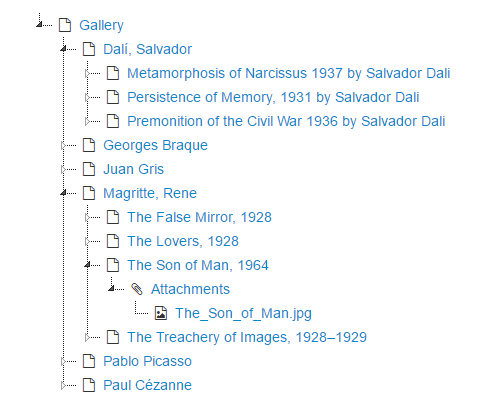
\includegraphics[scale=1.1]{img/docTree.png}
  \caption{Structura arborescentă a documentelor wiki}
\end{figure}
\clearpage

Pentru a putea parsa mai ușor conținutul unei pagini wiki am recurs la accesarea acestei în format xml, lucru posibil prin simpla apelare a acesteia cu parametrul \textit{xpage=xml}.
Acest lucru facilitează aplicației noastre izolarea și extragerea resurselor relevante cu ajutorul parserului xml.

\begin{figure}[h]
  \centering
  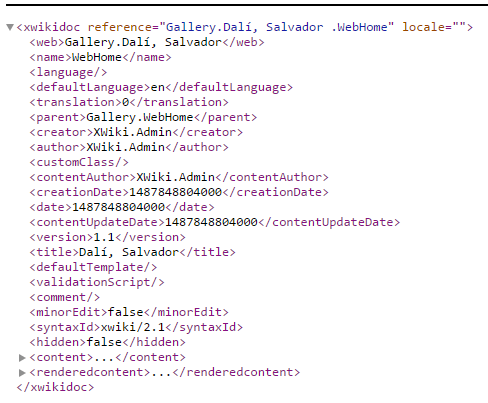
\includegraphics[scale=1.2]{img/xpagexml.png}
  \caption{Document wiki în format xml}
\end{figure}
\clearpage

URI-ul rădăcină a serviciului XWiki RESTful API este setat implicit la:

\textit{http://host:port/xwiki/rest}

Spre exemplu resursa \textit{/wikis} de pe un server ce rulează local pe portul 8080 poate fi accesată folosind următorul URL:

\textit{http://localhost:8080/xwiki/rest/wikis}

În cazul nostru am folosit acest serviciu pentru a determina copiii unei pagini. Conform documentației, URL-ul pentru a accesa acest tip de resursă va avea următoare formă:

\textit{/wikis/{wikiName}/spaces/{spaceName}[/spaces/{nestedSpaceName}]*/pages/{pageName}/children}

\begin{figure}[h]
  \centering
  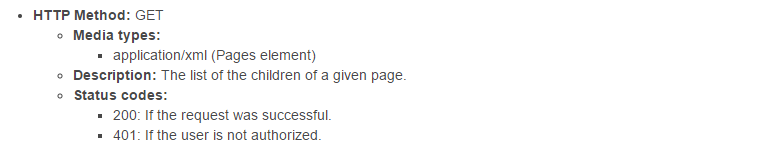
\includegraphics[scale=1]{img/restAPI.png}
\end{figure}

\section{Funcționalități de adăugat}

Deși dispozitivul Leap Motion este impresionant în abilitatea lui de a captura și transpune mâinile în obiecte virtuale, tehnologia este abia la început iar în practică, acuratețea acestui lasă de dorit. Din acest motiv, adăugarea suportului pentru metode de input mai precise, cum ar fi controlerele Vive sau Oculus Touch, va fi pe lista lucrurilor de adăugat în viitor.

O altă funcționalitate ce ar oferi un plus de valoare aplicației ar fi adăugarea posibilității mai multor persoane de a se conecta, întâlni și comunica în cadrul aceleași instanțe, lucru ce ar extinde considerabil aria de use case-uri.

\cleardoublepage
\chapter {Viziune}

\section{Control}

Găsirea unor noi forme fundamentale de interacțiune cu mediul virtual reprezintă următorul pas atât în evoluția tehnologiei cât și a societății. Apariția realității virtuale și cea augmentată viața publică a atras după sine interesul companiilor și a indivizilor de a utiliza și dezvolta aceste tehnologii, iar obstacolele întâmpinate în acest proces, ca efectul vertigo sau lipsa unor modalități de mișcare naturală încurajează creativitatea și inovația.

Lumea virtuală este la un pas de contopire cu lumea reală, cu companii ca Tesla, Facebook, Google ce au departamente dedicate cercetării și dezvoltării nu doar în domeniul VR/AR dar și al inteligenței artificiale sau neurociberneticii.

Dar nu doar corporații cu rezonanță apar pe lista celor care vor să transforme științifico-fantasticul în realitate, dar și companii mici și mijlocii, cum ar fi enigmatica companie start-up Magic Leap, ce promite introducerea unei tehnologii pe care ei o numesc \textit{mixt reality}, ce va înlocui ecranele standard.

\begin{figure}[h]
  \centering
  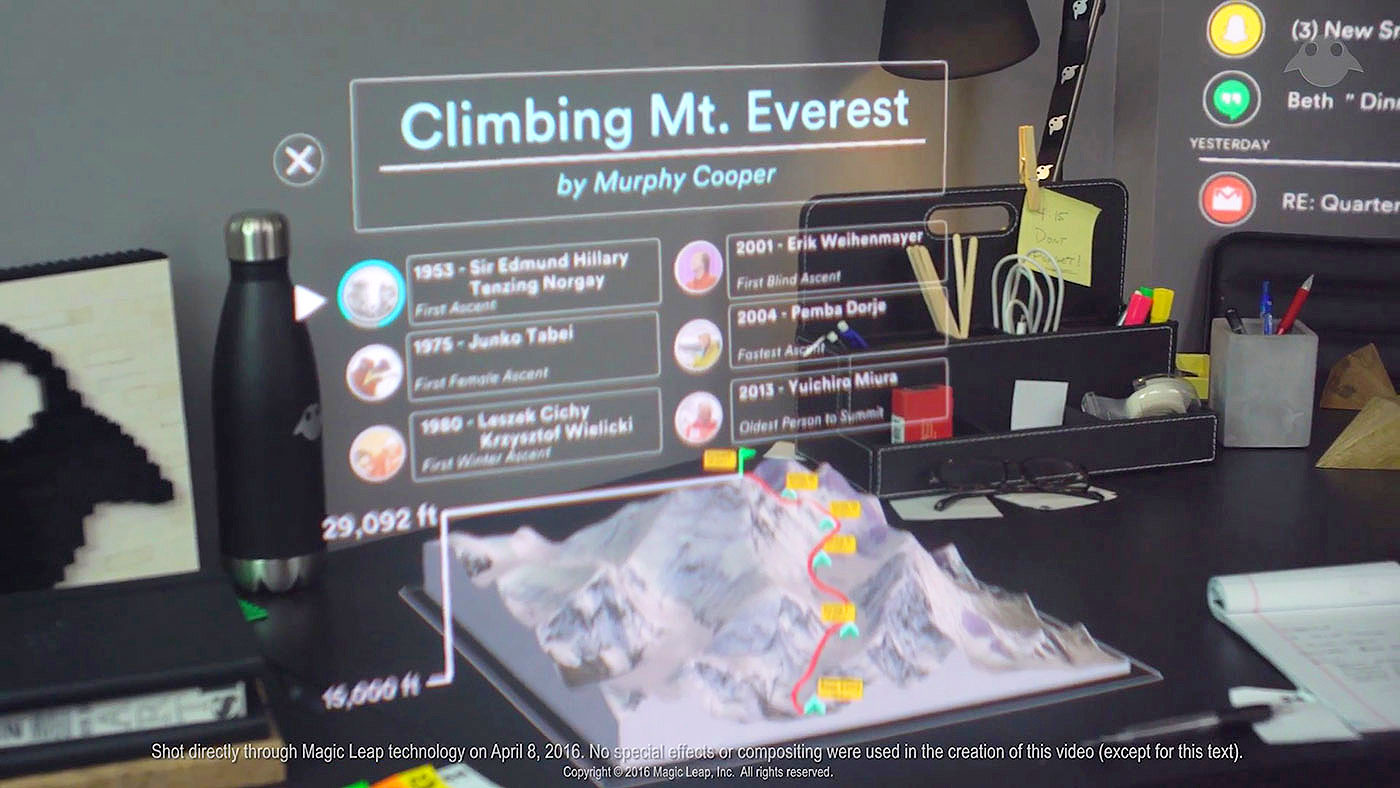
\includegraphics[scale=0.27]{img/magicleap.jpg}
  \caption{Imagine extrasă dintr-un clip demonstrativ distribuit de Magic Leap}
\end{figure}

O altă metodă tot mai populară de a controla aparatura din jurul nostru, este folosirea vocii pentru a vorbi direct cu acestea. Utilizarea comenzilor vocale pentru a interacționa cu telefonu mobil nu este ceva nou, dar gadgeturi ca Amazon Echo, Google Home și mai nou Apple HomePod, cu care putem controla lucruri obișnuite din casă ca becurile, televizorul și termostatul, promovează acest tip de interacțiune și transformă încă un element din universul Star Trek în realitate.

Progrese importante ce ar putea juca un rol extrem de important în viitorul nu foarte îndepărtat au fost făcute și în domeniul neuro-științei. Neurologii reușind să mapeze foarte detaliat cortexul cerebral (scoarța cerebrală), iar computerele devenind suficient de rapide pentru a detecta și interpreta semnalele creierului în timp real, este doar o chestiune de timp până vom putea controla tehnologia direct cu puterea gândului. 

Gândul este proces non-verbal și pur. Este mediul primar prin care ne controlăm corpul iar transformarea creierului  într-un controler direct al tehnologiei reprezintă idealul eficienței de comunicare cu dispozitivele pe care creăm.

Deși pare doar o fantezie această tehnologie deja există.
Compania Emotiv a lansat deja pe piață un astfel de dispozitiv ce poate controla spre exemplu o mașinuță electrică doar prin concentrarea asupra ideii de mișcare.
Dispozitivul este în principiu un mini-electroencefalograf  ce poate detecta undele cerebrale produse când ne concentrăm asupra unui lucru simplu și clar.

\begin{figure}[h]
  \centering
  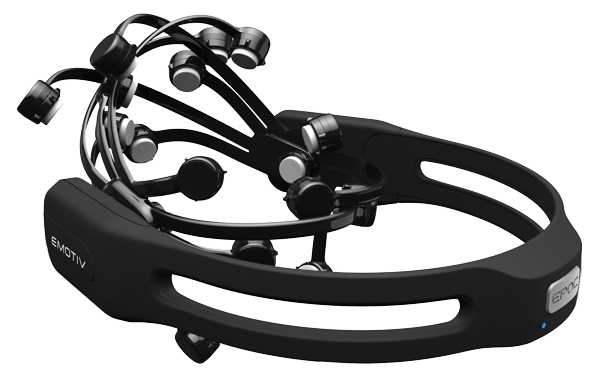
\includegraphics[scale=0.6]{img/emotiv_epoc.png}
  \caption{Dispozitivul Epoc+ dezvoltat de compania Emotiv}
\end{figure}
\newpage

\section{Brain-computer interface}

\textit{Brain-computer interface} prescurtat \textit{BCI}, uneori numit și \textit{mind-machine interface(MMI)} sau \textit{direct neural interface (DNI)} este o cale de comunicare directă între creier și un dispozitiv extern. BCI sunt adesea întrebuințate în cercetarea, maparea, asistarea, augmentarea sau repararea funcțiilor cognitive sau senzoriale ale omului.

Există trei tipuri de BCI:
\begin{itemize}
\item Invazive

\begin{figure}[h]
  \centering
  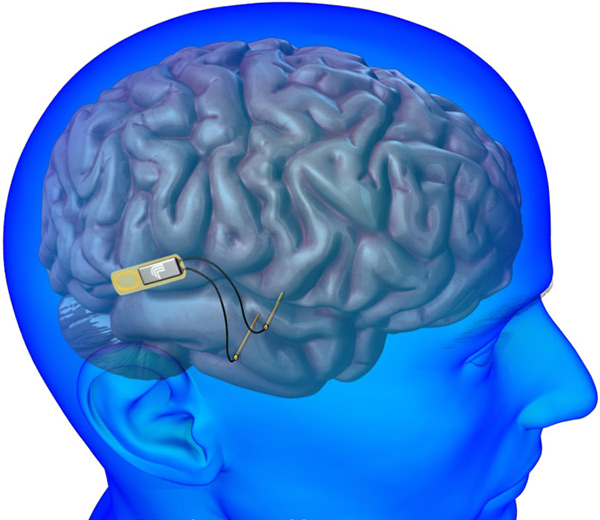
\includegraphics[scale=0.2]{img/invasiveBCI.jpg}
\end{figure}

Dispozitivul de transmitere a semnalelor este implantat direct în materia cenușie. Această metodă produce cea mai înaltă calitate a semnalelor dar acumularea de țesut cicatrizat poate duce la degradarea semnalelor.

\item Parțial invazive

\begin{figure}[h]
  \centering
  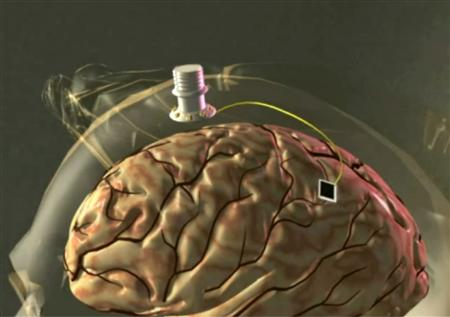
\includegraphics[scale=0.4]{img/BrainGate.jpg}
\end{figure}

Dispozitivul este implantat în interiorul craniului dar nu în țesutul cerebral. Produc semnale de o calitate mai înaltă calitate decât cele non-invazive prin atenuarea efectului inhibitor produs de craniu, și este mai puțin predispus la lezarea țesutului.

\item Non-invazive

\begin{figure}[h]
  \centering
  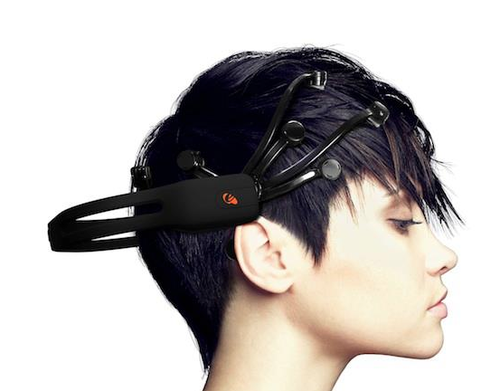
\includegraphics[scale=0.3]{img/noninvasiveBCI.png}
\end{figure}

Implică doar o cască ce înregistrează semnalele electromagnetice transmise de neuroni, fără nevoia niciunui implant. Deși această metodă este cea mai simplă, suferă de rezoluție slabă din cauza interferenței craniului cu semnalele.
\end{itemize}

Aceste tehnologii, în special cele non-intruzive sunt deja disponibile publicului. \textit{OpenBCI} spre exemplu este o companie dedicată să ofere tuturor accesul la date biometrice. Prin intermediul Kickstarter vor să lanseze un dispozitiv BCI open-source.

Alte proiecte ca \textit{Neural Lace}, dezvoltat de noua companie de cercetare medicală lansată de Elon Musk, Neuralink, au ca scop, inițial de a ajuta persoanele cu dizabilități neurologice, iar mai apoi de a augmenta creierul pentru a putea ține pasul cu progresul rapid al inteligenței artificiale.

\section{Singularitate tehnologică}

Singularitatea tehnologică este un concept din futurologie care se referă la implicațiile pe care în general le are progresul tehnico-științific foarte accelerat pentru specia umană și ceea ce înțelegem prin om.

Termenul a fost împrumutat din fizică unde singularitate este de exemplu o gaură neagră, oamenii neputând să afle ce este în interiorul ei, neputând pătrunde dincolo de raza Schwarzschild, legile fizicii nemaiavând valabilitate aici și din  matematică / analiza complexă unde singularitatea este punctul în care o ecuație sau o suprafață degenerează sau dispare.

Extrapolând legea lui Moore, Kurzweil presupune că în cei 100 de ani ai secolului al XXI-lea vom asista la o evoluție comparabilă cu 20.000 de ani precedenți, dacă se menține curba exponențială. Aceasta deoarece odată ce computerele vor depăși performanța creierului uman, ele vor fi capabile să se autoîmbunătățească, menținând ritmul de creștere exponențial al vitezei de calcul. Rezultatul va fi că progresul tehnico-științific va cunoaște o accelerare din ce în ce mai înaltă. Acele computere vor fi în stare până la urmă să descifreze aproape toate secretele naturii și Universului.

Acest presupus salt tehnologic ultrarapid va duce la evenimente aproape imposibil de imaginat pentru specia homo sapiens: contopirea dintre inteligența biologică și cea nebiologică (mind uploading), oameni aproape nemuritori și nivele înalte de superinteligență care se răspândesc rapid în întreg Universul. De aceea este folosit termenul de singularitate: specia umană nu are cum să înțeleagă ce va urma (gaură neagră), la fel cum o bacterie nu poate înțelege ce este un om, atât de mare va fi progresul tehnico-științific.

\bibliographystyle{plain}
\bibliography{osf}
\nocite{*}
\cleardoublepage
\tableofcontents	
\cleardoublepage
\listoffigures

\end{document}
